\documentclass[]{article}
\usepackage{lmodern}
\usepackage{amssymb,amsmath}
\usepackage{ifxetex,ifluatex}
\usepackage{fixltx2e} % provides \textsubscript
\ifnum 0\ifxetex 1\fi\ifluatex 1\fi=0 % if pdftex
  \usepackage[T1]{fontenc}
  \usepackage[utf8]{inputenc}
\else % if luatex or xelatex
  \ifxetex
    \usepackage{mathspec}
  \else
    \usepackage{fontspec}
  \fi
  \defaultfontfeatures{Ligatures=TeX,Scale=MatchLowercase}
\fi
% use upquote if available, for straight quotes in verbatim environments
\IfFileExists{upquote.sty}{\usepackage{upquote}}{}
% use microtype if available
\IfFileExists{microtype.sty}{%
\usepackage{microtype}
\UseMicrotypeSet[protrusion]{basicmath} % disable protrusion for tt fonts
}{}
\usepackage[margin=1in]{geometry}
\usepackage{hyperref}
\hypersetup{unicode=true,
            pdftitle={Introduction to Statistics},
            pdfborder={0 0 0},
            breaklinks=true}
\urlstyle{same}  % don't use monospace font for urls
\usepackage{color}
\usepackage{fancyvrb}
\newcommand{\VerbBar}{|}
\newcommand{\VERB}{\Verb[commandchars=\\\{\}]}
\DefineVerbatimEnvironment{Highlighting}{Verbatim}{commandchars=\\\{\}}
% Add ',fontsize=\small' for more characters per line
\usepackage{framed}
\definecolor{shadecolor}{RGB}{248,248,248}
\newenvironment{Shaded}{\begin{snugshade}}{\end{snugshade}}
\newcommand{\AlertTok}[1]{\textcolor[rgb]{0.94,0.16,0.16}{#1}}
\newcommand{\AnnotationTok}[1]{\textcolor[rgb]{0.56,0.35,0.01}{\textbf{\textit{#1}}}}
\newcommand{\AttributeTok}[1]{\textcolor[rgb]{0.77,0.63,0.00}{#1}}
\newcommand{\BaseNTok}[1]{\textcolor[rgb]{0.00,0.00,0.81}{#1}}
\newcommand{\BuiltInTok}[1]{#1}
\newcommand{\CharTok}[1]{\textcolor[rgb]{0.31,0.60,0.02}{#1}}
\newcommand{\CommentTok}[1]{\textcolor[rgb]{0.56,0.35,0.01}{\textit{#1}}}
\newcommand{\CommentVarTok}[1]{\textcolor[rgb]{0.56,0.35,0.01}{\textbf{\textit{#1}}}}
\newcommand{\ConstantTok}[1]{\textcolor[rgb]{0.00,0.00,0.00}{#1}}
\newcommand{\ControlFlowTok}[1]{\textcolor[rgb]{0.13,0.29,0.53}{\textbf{#1}}}
\newcommand{\DataTypeTok}[1]{\textcolor[rgb]{0.13,0.29,0.53}{#1}}
\newcommand{\DecValTok}[1]{\textcolor[rgb]{0.00,0.00,0.81}{#1}}
\newcommand{\DocumentationTok}[1]{\textcolor[rgb]{0.56,0.35,0.01}{\textbf{\textit{#1}}}}
\newcommand{\ErrorTok}[1]{\textcolor[rgb]{0.64,0.00,0.00}{\textbf{#1}}}
\newcommand{\ExtensionTok}[1]{#1}
\newcommand{\FloatTok}[1]{\textcolor[rgb]{0.00,0.00,0.81}{#1}}
\newcommand{\FunctionTok}[1]{\textcolor[rgb]{0.00,0.00,0.00}{#1}}
\newcommand{\ImportTok}[1]{#1}
\newcommand{\InformationTok}[1]{\textcolor[rgb]{0.56,0.35,0.01}{\textbf{\textit{#1}}}}
\newcommand{\KeywordTok}[1]{\textcolor[rgb]{0.13,0.29,0.53}{\textbf{#1}}}
\newcommand{\NormalTok}[1]{#1}
\newcommand{\OperatorTok}[1]{\textcolor[rgb]{0.81,0.36,0.00}{\textbf{#1}}}
\newcommand{\OtherTok}[1]{\textcolor[rgb]{0.56,0.35,0.01}{#1}}
\newcommand{\PreprocessorTok}[1]{\textcolor[rgb]{0.56,0.35,0.01}{\textit{#1}}}
\newcommand{\RegionMarkerTok}[1]{#1}
\newcommand{\SpecialCharTok}[1]{\textcolor[rgb]{0.00,0.00,0.00}{#1}}
\newcommand{\SpecialStringTok}[1]{\textcolor[rgb]{0.31,0.60,0.02}{#1}}
\newcommand{\StringTok}[1]{\textcolor[rgb]{0.31,0.60,0.02}{#1}}
\newcommand{\VariableTok}[1]{\textcolor[rgb]{0.00,0.00,0.00}{#1}}
\newcommand{\VerbatimStringTok}[1]{\textcolor[rgb]{0.31,0.60,0.02}{#1}}
\newcommand{\WarningTok}[1]{\textcolor[rgb]{0.56,0.35,0.01}{\textbf{\textit{#1}}}}
\usepackage{longtable,booktabs}
\usepackage{graphicx,grffile}
\makeatletter
\def\maxwidth{\ifdim\Gin@nat@width>\linewidth\linewidth\else\Gin@nat@width\fi}
\def\maxheight{\ifdim\Gin@nat@height>\textheight\textheight\else\Gin@nat@height\fi}
\makeatother
% Scale images if necessary, so that they will not overflow the page
% margins by default, and it is still possible to overwrite the defaults
% using explicit options in \includegraphics[width, height, ...]{}
\setkeys{Gin}{width=\maxwidth,height=\maxheight,keepaspectratio}
\IfFileExists{parskip.sty}{%
\usepackage{parskip}
}{% else
\setlength{\parindent}{0pt}
\setlength{\parskip}{6pt plus 2pt minus 1pt}
}
\setlength{\emergencystretch}{3em}  % prevent overfull lines
\providecommand{\tightlist}{%
  \setlength{\itemsep}{0pt}\setlength{\parskip}{0pt}}
\setcounter{secnumdepth}{5}
% Redefines (sub)paragraphs to behave more like sections
\ifx\paragraph\undefined\else
\let\oldparagraph\paragraph
\renewcommand{\paragraph}[1]{\oldparagraph{#1}\mbox{}}
\fi
\ifx\subparagraph\undefined\else
\let\oldsubparagraph\subparagraph
\renewcommand{\subparagraph}[1]{\oldsubparagraph{#1}\mbox{}}
\fi

%%% Use protect on footnotes to avoid problems with footnotes in titles
\let\rmarkdownfootnote\footnote%
\def\footnote{\protect\rmarkdownfootnote}

%%% Change title format to be more compact
\usepackage{titling}

% Create subtitle command for use in maketitle
\providecommand{\subtitle}[1]{
  \posttitle{
    \begin{center}\large#1\end{center}
    }
}

\setlength{\droptitle}{-2em}

  \title{Introduction to Statistics}
    \pretitle{\vspace{\droptitle}\centering\huge}
  \posttitle{\par}
    \author{}
    \preauthor{}\postauthor{}
    \date{}
    \predate{}\postdate{}
  

\begin{document}
\maketitle

{
\setcounter{tocdepth}{2}
\tableofcontents
}
\hypertarget{about-this-course}{%
\section*{About this course}\label{about-this-course}}
\addcontentsline{toc}{section}{About this course}

This course is an introduction to statistics, R and RStudio. Our primary aims are to introduce you to and help you become familiar with RStudio and quantitative methodologies critical to your development as an analyst.

By the end of the course, you should be able to understand fundamental research methods, apply them to real world problems and acquire competency in performing statistical functions using R.

\begin{center}\rule{0.5\linewidth}{\linethickness}\end{center}

Slides day 1

\hypertarget{introduction-to-r-and-rstudio}{%
\section{Introduction to R and RStudio}\label{introduction-to-r-and-rstudio}}

\hypertarget{learning-objectives}{%
\subsection{Learning objectives}\label{learning-objectives}}

In this session, we will have a look at R and RStudio. We will interact with both and use the various components of RStudio.

\hypertarget{what-is-r}{%
\subsubsection{What is R?}\label{what-is-r}}

R is an environment for statistical computing and graphics. RStudio is an editor or integrated development environment (IDE) that makes working with R much more comfortable.

To install R and RStudio on your computer, download both from the following sources:

\begin{itemize}
\tightlist
\item
  Download R from \href{https://cran.r-project.org}{The Comprehensive R Archive Network (CRAN)}
\item
  Download RStudio from \href{https://www.rstudio.com}{RStudio.com}
\end{itemize}

Keep both R and RStudio up to date. That means go online and check for newer versions. In case there are new versions, download those and re-install.

\hypertarget{rstudio}{%
\subsubsection{RStudio}\label{rstudio}}

Let's get acquainted with R. When you start RStudio for the first time, you'll see three panes:

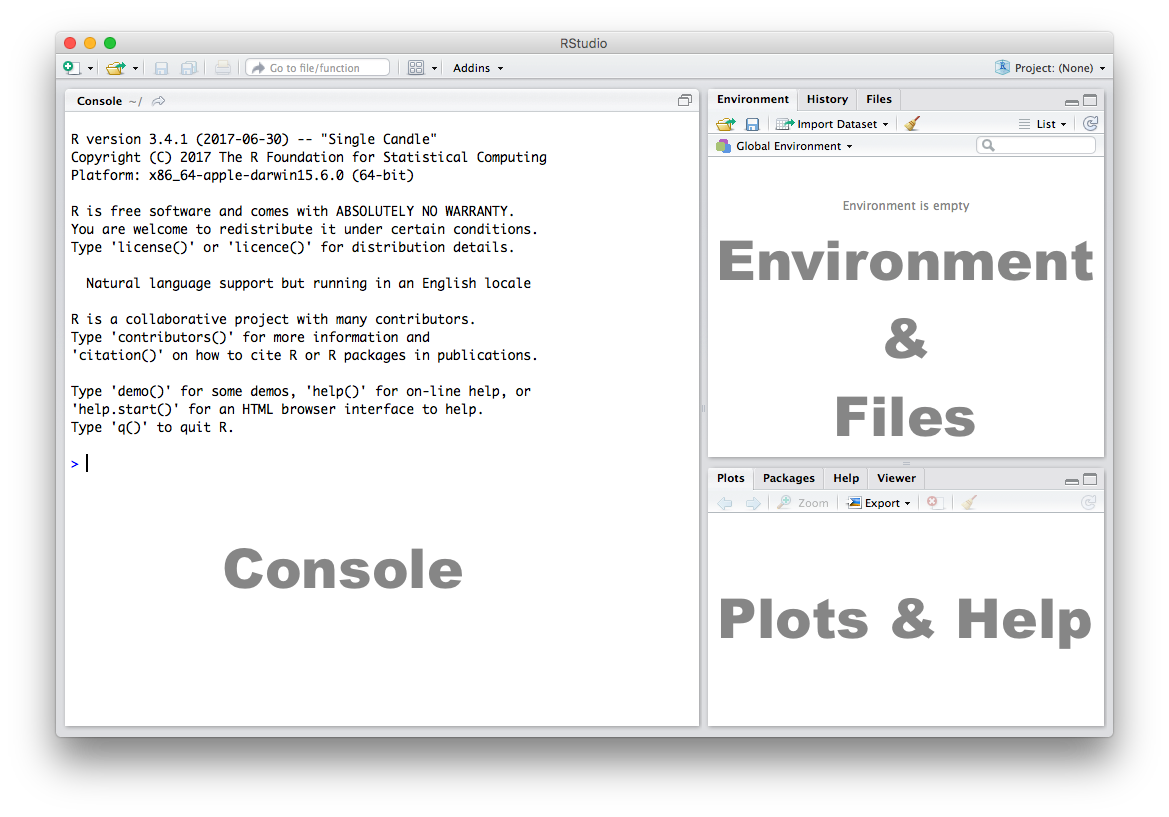
\includegraphics{./img/rstudio_default.png}

\hypertarget{console}{%
\subsubsection{Console}\label{console}}

The Console in RStudio is the simplest way to interact with R. You can type some code at the Console and when you press ENTER, R will run that code. Depending on what you type, you may see some output in the Console or if you make a mistake, you may get a warning or an error message.

Let's familiarize ourselves with the console by using R as a simple calculator:

\begin{Shaded}
\begin{Highlighting}[]
\DecValTok{2} \OperatorTok{+}\StringTok{ }\DecValTok{4}
\end{Highlighting}
\end{Shaded}

\begin{verbatim}
[1] 6
\end{verbatim}

Now that we know how to use the \texttt{+} sign for addition, let's try some other mathematical operations such as subtraction (\texttt{-}), multiplication (\texttt{*}), and division (\texttt{/}).

\begin{Shaded}
\begin{Highlighting}[]
\DecValTok{10} \OperatorTok{-}\StringTok{ }\DecValTok{4}
\end{Highlighting}
\end{Shaded}

\begin{verbatim}
[1] 6
\end{verbatim}

\begin{Shaded}
\begin{Highlighting}[]
\DecValTok{5} \OperatorTok{*}\StringTok{ }\DecValTok{3}
\end{Highlighting}
\end{Shaded}

\begin{verbatim}
[1] 15
\end{verbatim}

\begin{Shaded}
\begin{Highlighting}[]
\DecValTok{7} \OperatorTok{/}\StringTok{ }\DecValTok{2}
\end{Highlighting}
\end{Shaded}

\begin{verbatim}
[1] 3.5
\end{verbatim}

\begin{longtable}[]{@{}ll@{}}
\toprule
\endhead
\begin{minipage}[t]{0.69\columnwidth}\raggedright
You can use the cursor or arrow keys on your keyboard to edit your code at the console:- Use the UP and DOWN keys to re-run something without typing it again- Use the LEFT and RIGHT keys to edit\strut
\end{minipage} & \begin{minipage}[t]{0.25\columnwidth}\raggedright
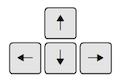
\includegraphics{./img/rstudio_cursorkeys.png}\strut
\end{minipage}\tabularnewline
\bottomrule
\end{longtable}

Take a few minutes to play around at the console and try different things out. Don't worry if you make a mistake, you can't break anything easily!

\hypertarget{scripts}{%
\subsubsection{Scripts}\label{scripts}}

The Console is great for simple tasks but if you're working on a project you would mostly likely want to save your work in some sort of a document or a file. Scripts in R are just plain text files that contain R code. You can edit a script just like you would edit a file in any word processing or note-taking application.

Create a new script using the menu or the toolbar button as shown below.

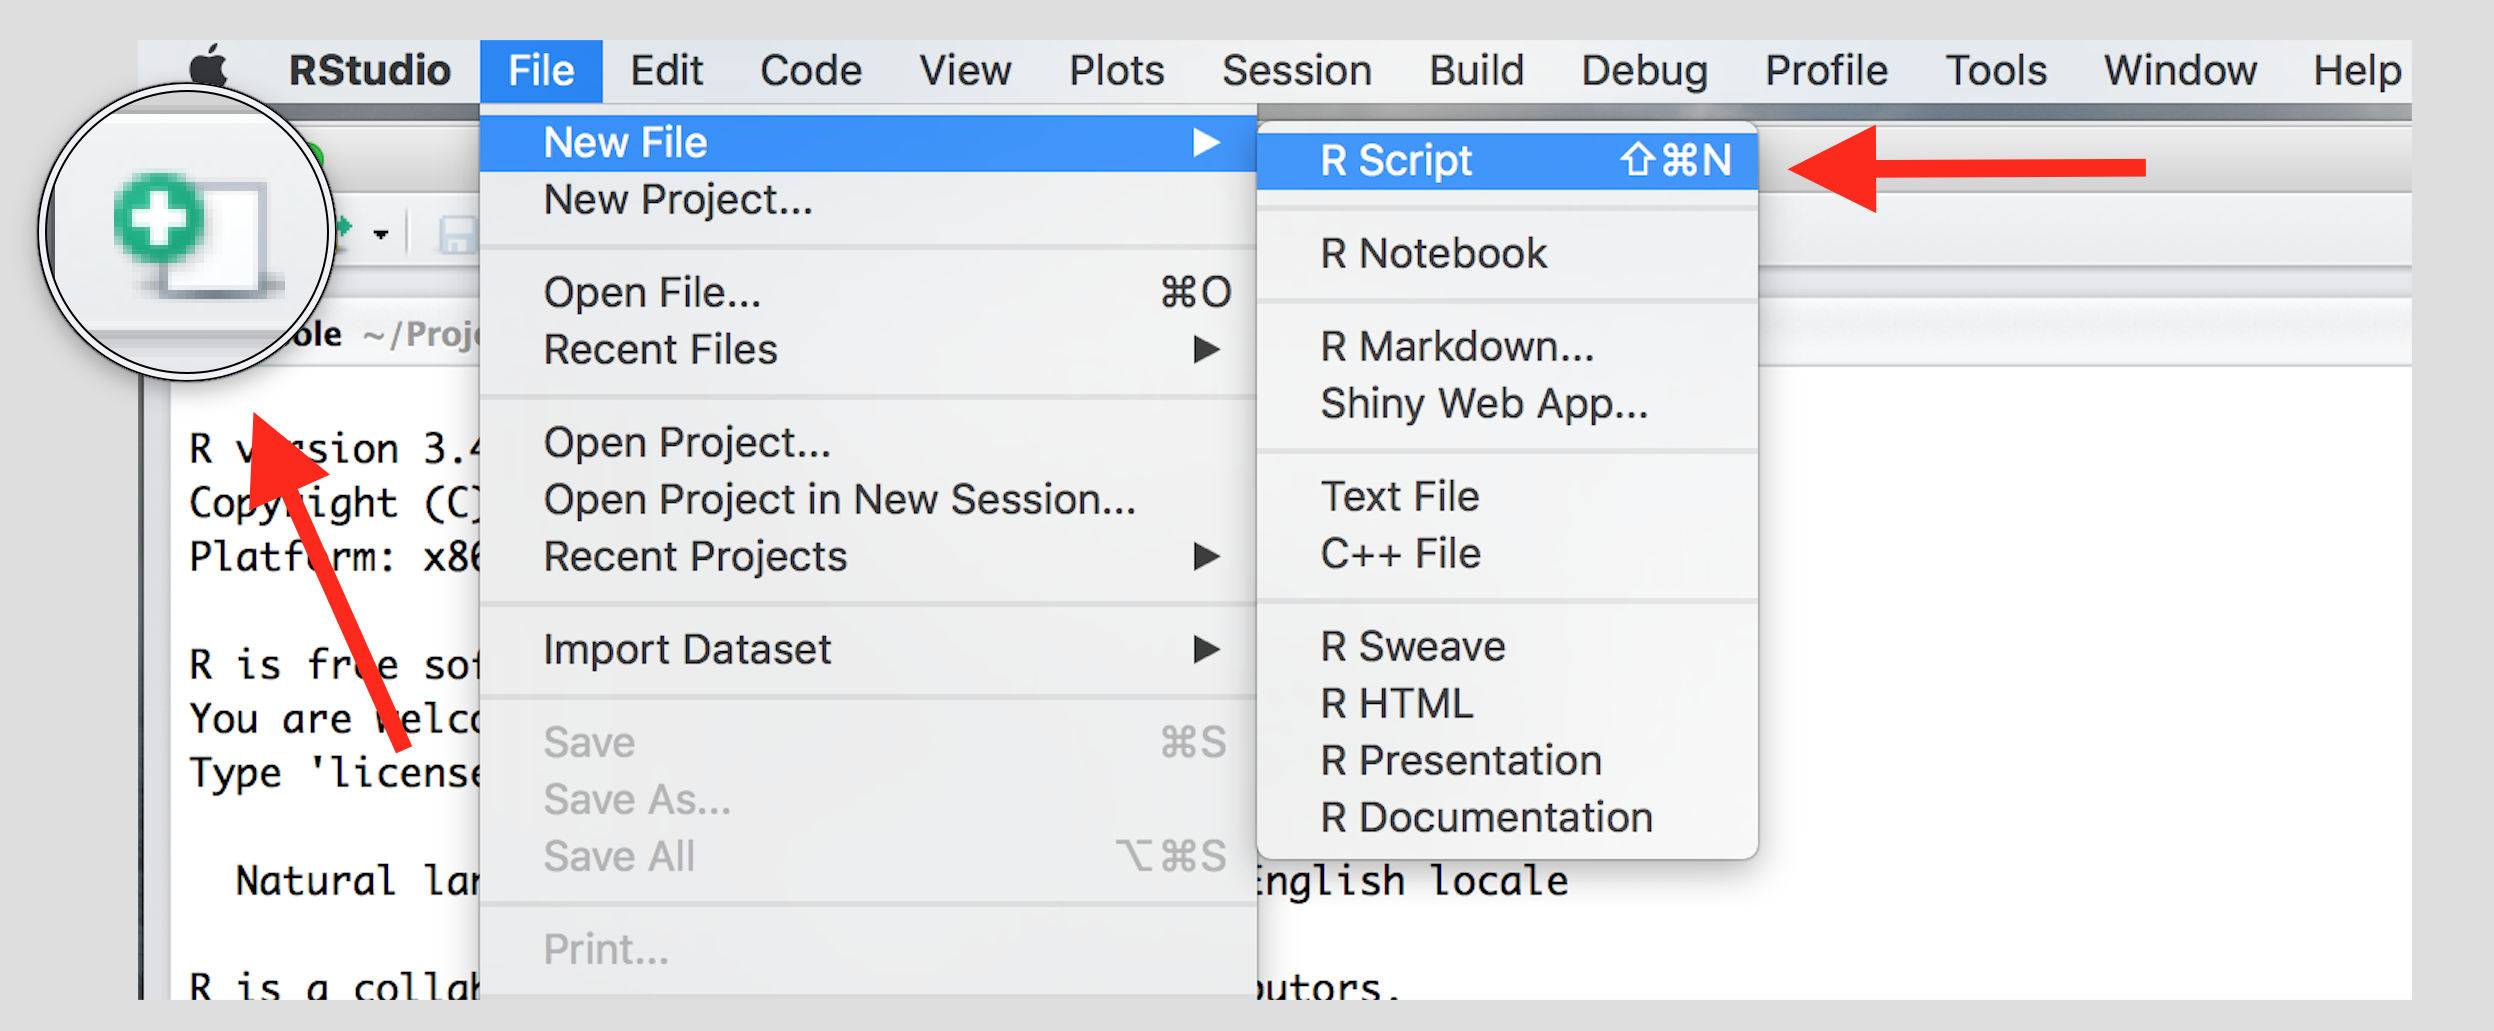
\includegraphics{./img/rstudio_newfile.png}

Once you've created a script, it is generally a good idea to give it a meaningful name and save it immediately. For our first session save your script as \textbf{seminar1.R}

\begin{longtable}[]{@{}ll@{}}
\toprule
\endhead
\begin{minipage}[t]{0.52\columnwidth}\raggedright
Familiarize yourself with the script window in RStudio, and especially the two buttons labeled \textbf{Run} and \textbf{Source}\strut
\end{minipage} & \begin{minipage}[t]{0.42\columnwidth}\raggedright
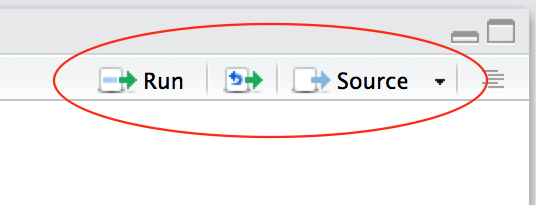
\includegraphics{./img/rstudio_script.png}\strut
\end{minipage}\tabularnewline
\bottomrule
\end{longtable}

There are a few different ways to run your code from a script.

\begin{longtable}[]{@{}ll@{}}
\toprule
\endhead
\begin{minipage}[t]{0.23\columnwidth}\raggedright
One line at a time\strut
\end{minipage} & \begin{minipage}[t]{0.71\columnwidth}\raggedright
Place the cursor on the line you want to run and hit CTRL-ENTER or use the \textbf{Run} button\strut
\end{minipage}\tabularnewline
\begin{minipage}[t]{0.23\columnwidth}\raggedright
Multiple lines\strut
\end{minipage} & \begin{minipage}[t]{0.71\columnwidth}\raggedright
Select the lines you want to run and hit CTRL-ENTER or use the \textbf{Run} button\strut
\end{minipage}\tabularnewline
\begin{minipage}[t]{0.23\columnwidth}\raggedright
Entire script\strut
\end{minipage} & \begin{minipage}[t]{0.71\columnwidth}\raggedright
Use the \textbf{Source} button\strut
\end{minipage}\tabularnewline
\bottomrule
\end{longtable}

\hypertarget{data-stuctures-and-data-types}{%
\section{Data Stuctures and Data Types}\label{data-stuctures-and-data-types}}

\hypertarget{seminar}{%
\subsection{Seminar}\label{seminar}}

In this session we introduce R-syntax, and data types.

\hypertarget{functions}{%
\subsubsection{Functions}\label{functions}}

Functions are a set of instructions that carry out a specific task. Functions often require some input and generate some output. For example, instead of using the \texttt{+} operator for addition, we can use the \texttt{sum} function to add two or more numbers.

\begin{Shaded}
\begin{Highlighting}[]
\KeywordTok{sum}\NormalTok{(}\DecValTok{1}\NormalTok{, }\DecValTok{4}\NormalTok{, }\DecValTok{10}\NormalTok{)}
\end{Highlighting}
\end{Shaded}

\begin{verbatim}
[1] 15
\end{verbatim}

In the example above, \texttt{1,\ 4,\ 10} are the inputs and 15 is the output. A function always requires the use of parenthesis or round brackets \texttt{()}. Inputs to the function are called \textbf{arguments} and go inside the brackets. The output of a function is displayed on the screen but we can also have the option of saving the result of the output. More on this later.

\hypertarget{getting-help}{%
\subsubsection{Getting Help}\label{getting-help}}

Another useful function in R is \texttt{help} which we can use to display online documentation. For example, if we wanted to know how to use the \texttt{sum} function, we could type \texttt{help(sum)} and look at the online documentation.

\begin{Shaded}
\begin{Highlighting}[]
\KeywordTok{help}\NormalTok{(sum)}
\end{Highlighting}
\end{Shaded}

The question mark \texttt{?} can also be used as a shortcut to access online help.

\begin{Shaded}
\begin{Highlighting}[]
\NormalTok{?sum}
\end{Highlighting}
\end{Shaded}

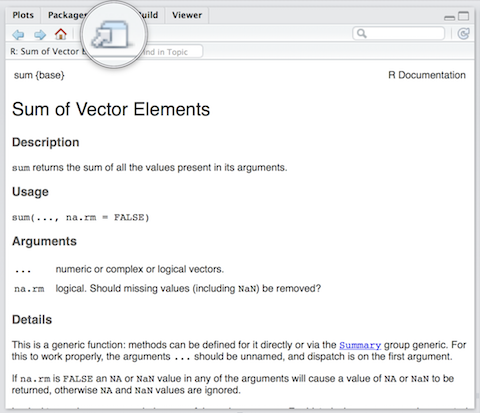
\includegraphics{./img/rstudio_help.png}

Use the toolbar button shown in the picture above to expand and display the help in a new window.

Help pages for functions in R follow a consistent layout generally include these sections:

\begin{longtable}[]{@{}ll@{}}
\toprule
\endhead
Description & A brief description of the function\tabularnewline
Usage & The complete syntax or grammar including all arguments (inputs)\tabularnewline
Arguments & Explanation of each argument\tabularnewline
Details & Any relevant details about the function and its arguments\tabularnewline
Value & The output value of the function\tabularnewline
Examples & Example of how to use the function\tabularnewline
\bottomrule
\end{longtable}

\hypertarget{the-assignment-operator}{%
\subsubsection{The Assignment Operator}\label{the-assignment-operator}}

Now we know how to provide inputs to a function using parenthesis or round brackets \texttt{()}, but what about the output of a function?

We use the assignment operator \textbf{\texttt{\textless{}-}} for creating or updating objects. If we wanted to save the result of adding \texttt{sum(1,\ 4,\ 10)}, we would do the following:

\begin{Shaded}
\begin{Highlighting}[]
\NormalTok{myresult <-}\StringTok{ }\KeywordTok{sum}\NormalTok{(}\DecValTok{1}\NormalTok{, }\DecValTok{4}\NormalTok{, }\DecValTok{10}\NormalTok{)}
\end{Highlighting}
\end{Shaded}

The line above creates a new object called \texttt{myresult} in our environment and saves the result of the \texttt{sum(1,\ 4,\ 10)} in it. To see what's in \texttt{myresult}, just type it at the console:

\begin{Shaded}
\begin{Highlighting}[]
\NormalTok{myresult}
\end{Highlighting}
\end{Shaded}

\begin{verbatim}
[1] 15
\end{verbatim}

Take a look at the \textbf{Environment} pane in RStudio and you'll see \texttt{myresult} there.

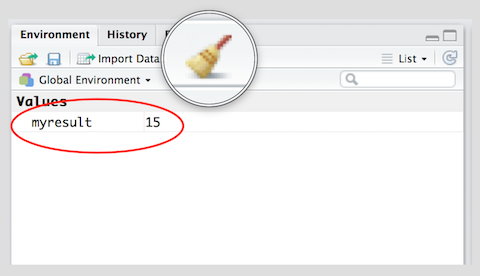
\includegraphics{./img/rstudio_env.png}

To delete all objects from the environment, you can use the \textbf{broom} button as shown in the picture above.

We called our object \texttt{myresult} but we can call it anything as long as we follow a few simple rules. Object names can contain upper or lower case letters (\texttt{A-Z}, \texttt{a-z}), numbers (\texttt{0-9}), underscores (\texttt{\_}) or a dot (\texttt{.}) but all object names must start with a letter. Choose names that are descriptive and easy to type.

\begin{longtable}[]{@{}ll@{}}
\toprule
Good Object Names & Bad Object Names\tabularnewline
\midrule
\endhead
result & a\tabularnewline
myresult & x1\tabularnewline
my.result & this.name.is.just.too.long\tabularnewline
my\_result &\tabularnewline
data1 &\tabularnewline
\bottomrule
\end{longtable}

\hypertarget{vectors-and-subsetting}{%
\subsubsection{Vectors and subsetting}\label{vectors-and-subsetting}}

A vector is one dimensional. It can contain one element in which case it is also called a scalar or many elements. We can add and multiply vectors. Think of a vector as a row or column in your excel spreadsheet.

To create a vector, we use the \texttt{c()} function, where c stands for collect. We start by creating a numeric vector.

\begin{Shaded}
\begin{Highlighting}[]
\NormalTok{vec1 <-}\StringTok{ }\KeywordTok{c}\NormalTok{(}\DecValTok{10}\NormalTok{, }\DecValTok{47}\NormalTok{, }\DecValTok{99}\NormalTok{, }\DecValTok{34}\NormalTok{, }\DecValTok{21}\NormalTok{)}
\end{Highlighting}
\end{Shaded}

Creating a character vector works in the same way. We need to use quotation marks to indicate that the data type is textual data.

\begin{Shaded}
\begin{Highlighting}[]
\NormalTok{vec2 <-}\StringTok{ }\KeywordTok{c}\NormalTok{(}\StringTok{"Emilia"}\NormalTok{, }\StringTok{"Martin"}\NormalTok{, }\StringTok{"Agatha"}\NormalTok{, }\StringTok{"James"}\NormalTok{, }\StringTok{"Luke"}\NormalTok{, }\StringTok{"Jacques"}\NormalTok{)}
\end{Highlighting}
\end{Shaded}

Let's see how many elements our vector contains using the \texttt{length()} function.

\begin{Shaded}
\begin{Highlighting}[]
\KeywordTok{length}\NormalTok{(vec1)}
\end{Highlighting}
\end{Shaded}

\begin{verbatim}
[1] 5
\end{verbatim}

\begin{Shaded}
\begin{Highlighting}[]
\KeywordTok{length}\NormalTok{(vec2)}
\end{Highlighting}
\end{Shaded}

\begin{verbatim}
[1] 6
\end{verbatim}

We need one coordinate to identify a unique element in a vector. For instance, we may be interested in the first element of the vector only. We use square brackets \texttt{{[}{]}} to access a specific element. The number in square brackets is the vector element that we wish to see.

\begin{Shaded}
\begin{Highlighting}[]
\NormalTok{vec1[}\DecValTok{1}\NormalTok{]}
\end{Highlighting}
\end{Shaded}

\begin{verbatim}
[1] 10
\end{verbatim}

To access all elements except the first element, we use the \texttt{-} operator

\begin{Shaded}
\begin{Highlighting}[]
\NormalTok{vec1[}\OperatorTok{-}\DecValTok{1}\NormalTok{]}
\end{Highlighting}
\end{Shaded}

\begin{verbatim}
[1] 47 99 34 21
\end{verbatim}

We can access elements 2 to 4 by using the colon \texttt{:} operator.

\begin{Shaded}
\begin{Highlighting}[]
\NormalTok{vec1[}\DecValTok{2}\OperatorTok{:}\DecValTok{4}\NormalTok{]}
\end{Highlighting}
\end{Shaded}

\begin{verbatim}
[1] 47 99 34
\end{verbatim}

We can access non-adjacent elements bu using the collect function \texttt{c()}.

\begin{Shaded}
\begin{Highlighting}[]
\NormalTok{vec1[}\KeywordTok{c}\NormalTok{(}\DecValTok{2}\NormalTok{,}\DecValTok{5}\NormalTok{)]}
\end{Highlighting}
\end{Shaded}

\begin{verbatim}
[1] 47 21
\end{verbatim}

Finally, we combine the \texttt{length()} function with the square brackets to access the last element in our vector.

\begin{Shaded}
\begin{Highlighting}[]
\NormalTok{vec1[ }\KeywordTok{length}\NormalTok{(vec1) ]}
\end{Highlighting}
\end{Shaded}

\begin{verbatim}
[1] 21
\end{verbatim}

\hypertarget{matrices}{%
\subsubsection{Matrices}\label{matrices}}

A matrix has two dimensions and stores data of the same type, e.g.~numbers or text but never both. A matrix is always rectangular. Think of it as your excel spreadsheet - essentially, it is a data table.

We create a matrix using the \texttt{matrix()} function. We need to provide the following arguments:

\begin{Shaded}
\begin{Highlighting}[]
\NormalTok{mat1 <-}\StringTok{ }\KeywordTok{matrix}\NormalTok{(}
  \DataTypeTok{data =} \KeywordTok{c}\NormalTok{(}\DecValTok{99}\NormalTok{, }\DecValTok{17}\NormalTok{, }\DecValTok{19}\NormalTok{, }\DecValTok{49}\NormalTok{, }\DecValTok{88}\NormalTok{, }\DecValTok{54}\NormalTok{),}
  \DataTypeTok{nrow =} \DecValTok{2}\NormalTok{,}
  \DataTypeTok{ncol =} \DecValTok{3}\NormalTok{,}
  \DataTypeTok{byrow =} \OtherTok{TRUE}
\NormalTok{)}
\end{Highlighting}
\end{Shaded}

\begin{longtable}[]{@{}ll@{}}
\toprule
Argument & Description\tabularnewline
\midrule
\endhead
data & the data in the matrix\tabularnewline
nrow & number of rows\tabularnewline
ncol & number of columns\tabularnewline
byrow & TRUE = matrix is filled rowwise\tabularnewline
\bottomrule
\end{longtable}

To display the matrix, we simply call the object by its name (in this case mat1).

\begin{Shaded}
\begin{Highlighting}[]
\NormalTok{mat1}
\end{Highlighting}
\end{Shaded}

\begin{verbatim}
     [,1] [,2] [,3]
[1,]   99   17   19
[2,]   49   88   54
\end{verbatim}

To access a unique element in a matrix, we need 2 coordinates. First, a row coordinate and second, a column coordinate. We use square brackets and separate the coordinates with a comma \texttt{{[}\ ,\ {]}}. The row coordinate goes before the comma and the column coordinate after.

We can access the the second row and third column like so:

\begin{Shaded}
\begin{Highlighting}[]
\NormalTok{mat1[}\DecValTok{2}\NormalTok{, }\DecValTok{3}\NormalTok{]}
\end{Highlighting}
\end{Shaded}

\begin{verbatim}
[1] 54
\end{verbatim}

To display an entire column, we specify the column we want to display and leave the row coordinate empty like so:

\begin{Shaded}
\begin{Highlighting}[]
\CommentTok{# display the 2nd column}
\NormalTok{mat1[ , }\DecValTok{2}\NormalTok{]}
\end{Highlighting}
\end{Shaded}

\begin{verbatim}
[1] 17 88
\end{verbatim}

Similarly, to display the entire second row, we specify the row coordinate but leave the column coordinate empty.

\begin{Shaded}
\begin{Highlighting}[]
\NormalTok{mat1[}\DecValTok{2}\NormalTok{, ]}
\end{Highlighting}
\end{Shaded}

\begin{verbatim}
[1] 49 88 54
\end{verbatim}

\hypertarget{arrays}{%
\subsubsection{Arrays}\label{arrays}}

Arrays are similar to matrices but can contain more dimensions. You can think of an array as stacking multiple matrices. Generally, we refer to the rows, columns and layers in array. Let's create an array with 2 rows, 3 columns and 4 layers using the \texttt{array()} function.

\begin{Shaded}
\begin{Highlighting}[]
\NormalTok{arr1 <-}\StringTok{ }\KeywordTok{array}\NormalTok{(}
  \DataTypeTok{data =} \KeywordTok{c}\NormalTok{(}\DecValTok{1}\OperatorTok{:}\DecValTok{24}\NormalTok{),}
  \DataTypeTok{dim =} \KeywordTok{c}\NormalTok{(}\DecValTok{2}\NormalTok{, }\DecValTok{3}\NormalTok{, }\DecValTok{4}\NormalTok{)}
\NormalTok{)}
\end{Highlighting}
\end{Shaded}

To display the object, we call it by its name.

\begin{Shaded}
\begin{Highlighting}[]
\NormalTok{arr1}
\end{Highlighting}
\end{Shaded}

\begin{verbatim}
, , 1

     [,1] [,2] [,3]
[1,]    1    3    5
[2,]    2    4    6

, , 2

     [,1] [,2] [,3]
[1,]    7    9   11
[2,]    8   10   12

, , 3

     [,1] [,2] [,3]
[1,]   13   15   17
[2,]   14   16   18

, , 4

     [,1] [,2] [,3]
[1,]   19   21   23
[2,]   20   22   24
\end{verbatim}

We can subset an array using the square brackets \texttt{{[}{]}}. To access a single element we need as many coordinates as our object has dimensions. Let's check the number of dimensions in our object first.

\begin{Shaded}
\begin{Highlighting}[]
\KeywordTok{dim}\NormalTok{(arr1)}
\end{Highlighting}
\end{Shaded}

\begin{verbatim}
[1] 2 3 4
\end{verbatim}

The \texttt{dim()} function informs us that we have 3 dimensions. The first is of length 2, the second of length 3 and the fourth of length 4.

Access the second column of the third layer on your own.

\begin{Shaded}
\begin{Highlighting}[]
\NormalTok{arr1[ , }\DecValTok{2}\NormalTok{, }\DecValTok{3}\NormalTok{] }
\end{Highlighting}
\end{Shaded}

\begin{verbatim}
[1] 15 16
\end{verbatim}

\hypertarget{creating-and-exploring-data-frames}{%
\section{Creating and Exploring Data Frames}\label{creating-and-exploring-data-frames}}

\hypertarget{seminar-1}{%
\subsection{Seminar}\label{seminar-1}}

In this session we introduce data frames using R-syntax.

\hypertarget{clearing-your-workspace-from-previous-work}{%
\subsubsection{Clearing your workspace from previous work}\label{clearing-your-workspace-from-previous-work}}

To remove a specific object or in this case a matrix, we can use the following command.

\begin{Shaded}
\begin{Highlighting}[]
\KeywordTok{ls}\NormalTok{()}
\end{Highlighting}
\end{Shaded}

\begin{verbatim}
[1] "chapter_header"
\end{verbatim}

\begin{Shaded}
\begin{Highlighting}[]
\KeywordTok{rm}\NormalTok{(mat1)}
\end{Highlighting}
\end{Shaded}

\begin{verbatim}
Warning in rm(mat1): object 'mat1' not found
\end{verbatim}

Otherwise we can remove everything, which is good practice when starting new work. The same can also be achieved by clicking on the yellow broomstick in the Enviornemnt and Files Panel in R Studio (top right hand panel)

\begin{Shaded}
\begin{Highlighting}[]
\KeywordTok{rm}\NormalTok{( }\DataTypeTok{list =} \KeywordTok{ls}\NormalTok{() )}
\end{Highlighting}
\end{Shaded}

\hypertarget{creating-data-frames}{%
\subsubsection{Creating data frames}\label{creating-data-frames}}

A data frame is an object that holds data in a tabular format similar to how spreadsheets work. Variables are generally kept in columns and observations are in rows. Data frames are similar to matrices but they can store vectors of different types (e.g.~numbers and text).

We start by creating a data frame with the \texttt{data.frame()} function. We will give each column a name (a variable name) followed by the \texttt{=} operator and the respective vector of data that we want to assign to that column.

\begin{Shaded}
\begin{Highlighting}[]
\NormalTok{england <-}\StringTok{ }\KeywordTok{data.frame}\NormalTok{(}
  \DataTypeTok{name =} \KeywordTok{c}\NormalTok{(}\StringTok{"South East"}\NormalTok{, }\StringTok{"London"}\NormalTok{, }\StringTok{"North West"}\NormalTok{, }\StringTok{"East of England"}\NormalTok{, }\StringTok{"West Midlands"}\NormalTok{, }\StringTok{"South West"}\NormalTok{,}
           \StringTok{"Yorkshire and the Humber"}\NormalTok{, }\StringTok{"East Midlands"}\NormalTok{, }\StringTok{"North East"}\NormalTok{),}
  \DataTypeTok{population =} \KeywordTok{c}\NormalTok{(}\FloatTok{8.6}\NormalTok{, }\FloatTok{8.2}\NormalTok{, }\FloatTok{7.1}\NormalTok{, }\FloatTok{5.9}\NormalTok{, }\FloatTok{5.6}\NormalTok{, }\FloatTok{5.3}\NormalTok{, }\FloatTok{5.3}\NormalTok{, }\FloatTok{4.5}\NormalTok{, }\FloatTok{2.6}\NormalTok{),}
  \DataTypeTok{earnings =} \KeywordTok{c}\NormalTok{(}\FloatTok{28.7}\NormalTok{, }\FloatTok{35.1}\NormalTok{, }\FloatTok{25.2}\NormalTok{, }\FloatTok{26.6}\NormalTok{, }\FloatTok{24.9}\NormalTok{, }\FloatTok{25.6}\NormalTok{, }\DecValTok{25}\NormalTok{, }\DecValTok{25}\NormalTok{, }\DecValTok{25}\NormalTok{)}
\NormalTok{)}
\end{Highlighting}
\end{Shaded}

We can also display the entire dataset in spreadsheet view by clicking on the object name in the environment window.

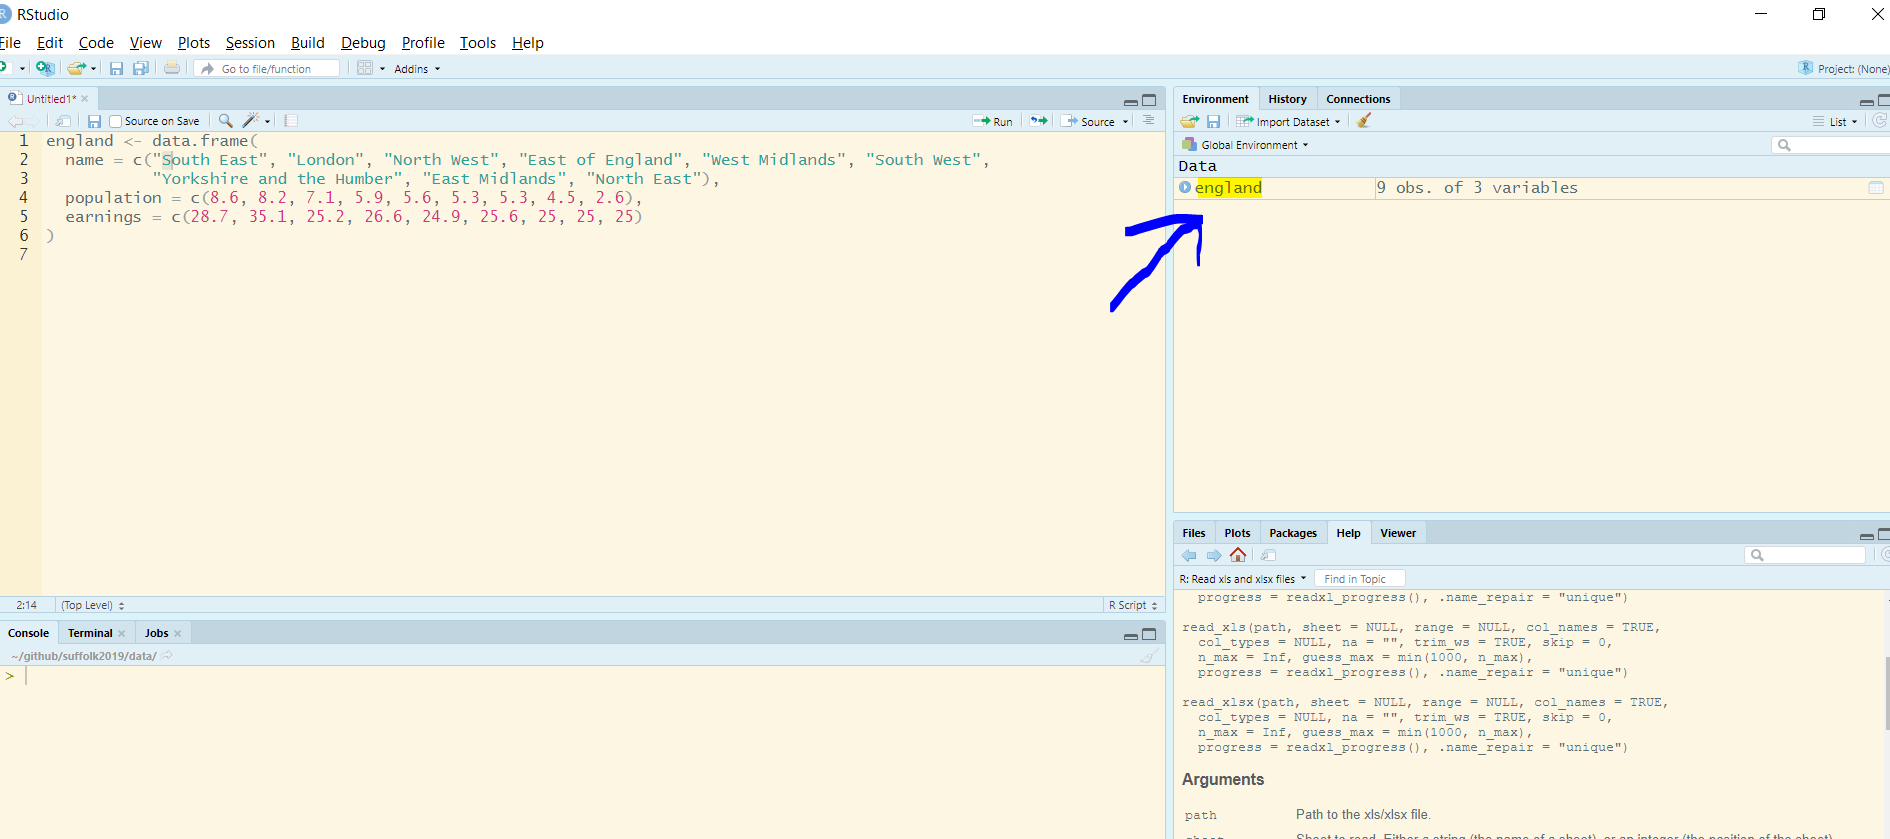
\includegraphics{./img/dataframe_in_spreadsheet_view.png}

\hypertarget{working-with-data-frames}{%
\subsubsection{Working with data frames}\label{working-with-data-frames}}

we can display the entire dataset in spreadsheet view by clicking on the object name in the environment window.

Alternatively, you can call the object name to display the dataset in the console window. Let's do so:

\begin{Shaded}
\begin{Highlighting}[]
\NormalTok{england}
\end{Highlighting}
\end{Shaded}

\begin{verbatim}
                      name population earnings
1               South East        8.6     28.7
2                   London        8.2     35.1
3               North West        7.1     25.2
4          East of England        5.9     26.6
5            West Midlands        5.6     24.9
6               South West        5.3     25.6
7 Yorkshire and the Humber        5.3     25.0
8            East Midlands        4.5     25.0
9               North East        2.6     25.0
\end{verbatim}

Often, datasets are too long to be viewed to in the console window. It is a good idea to look at the first couple of rows of a datasets to get an overview of its contents. We use the square brackets \texttt{{[}{]}} to view the first five rows and all columns.

\begin{Shaded}
\begin{Highlighting}[]
\NormalTok{england[}\DecValTok{1}\OperatorTok{:}\DecValTok{5}\NormalTok{, ]}
\end{Highlighting}
\end{Shaded}

\begin{verbatim}
             name population earnings
1      South East        8.6     28.7
2          London        8.2     35.1
3      North West        7.1     25.2
4 East of England        5.9     26.6
5   West Midlands        5.6     24.9
\end{verbatim}

v
Columns in a dataframe have names. We will often need to know the name of a column/variable to access it. We use the \texttt{names()} function to view all variable names in a dataframe.

\begin{Shaded}
\begin{Highlighting}[]
\KeywordTok{names}\NormalTok{(england)}
\end{Highlighting}
\end{Shaded}

\begin{verbatim}
[1] "name"       "population" "earnings"  
\end{verbatim}

We can access the earnings variable in multiple ways. First, we can use the \texttt{\$} operator. We write the name of the dataset object, followed by the \texttt{\$}, followed by the variable name like so:

\begin{Shaded}
\begin{Highlighting}[]
\NormalTok{england}\OperatorTok{$}\NormalTok{population}
\end{Highlighting}
\end{Shaded}

\begin{verbatim}
[1] 8.6 8.2 7.1 5.9 5.6 5.3 5.3 4.5 2.6
\end{verbatim}

We can also use the square brackets to access the earnings column.

\begin{Shaded}
\begin{Highlighting}[]
\NormalTok{england[, }\StringTok{"population"}\NormalTok{ ]}
\end{Highlighting}
\end{Shaded}

\begin{verbatim}
[1] 8.6 8.2 7.1 5.9 5.6 5.3 5.3 4.5 2.6
\end{verbatim}

The square brackets are sometimes preferred because we could access multiple columns at once like so:

\begin{Shaded}
\begin{Highlighting}[]
\NormalTok{england[, }\KeywordTok{c}\NormalTok{(}\StringTok{"name"}\NormalTok{, }\StringTok{"population"}\NormalTok{) ]}
\end{Highlighting}
\end{Shaded}

\begin{verbatim}
                      name population
1               South East        8.6
2                   London        8.2
3               North West        7.1
4          East of England        5.9
5            West Midlands        5.6
6               South West        5.3
7 Yorkshire and the Humber        5.3
8            East Midlands        4.5
9               North East        2.6
\end{verbatim}

You can also explore the variable further. For instance, calculate the average population in England and then select regions that have a population higher than this average. Again the dataset object is followed by the \texttt{\$}and then the variable name like so

\begin{Shaded}
\begin{Highlighting}[]
\KeywordTok{mean}\NormalTok{(england}\OperatorTok{$}\NormalTok{population)}
\end{Highlighting}
\end{Shaded}

\begin{verbatim}
[1] 5.9
\end{verbatim}

\begin{Shaded}
\begin{Highlighting}[]
\NormalTok{avg.pop =}\StringTok{ }\KeywordTok{mean}\NormalTok{(england}\OperatorTok{$}\NormalTok{population)}
\NormalTok{england [england}\OperatorTok{$}\NormalTok{population }\OperatorTok{>}\StringTok{ }\NormalTok{avg.pop,}
         \KeywordTok{c}\NormalTok{(}\StringTok{"name"}\NormalTok{, }\StringTok{"population"}\NormalTok{)]}
\end{Highlighting}
\end{Shaded}

\begin{verbatim}
             name population
1      South East        8.6
2          London        8.2
3      North West        7.1
4 East of England        5.9
\end{verbatim}

Variables come in different types such as numbers, text, logical (true/false). We need to know the type of a variable because the type affects statistical analysis. We use the \texttt{str()} function to check the type of each variable in our dataset.

\begin{Shaded}
\begin{Highlighting}[]
\KeywordTok{str}\NormalTok{(england)}
\end{Highlighting}
\end{Shaded}

\begin{verbatim}
'data.frame':   9 obs. of  3 variables:
 $ name      : Factor w/ 9 levels "East Midlands",..: 6 3 5 2 8 7 9 1 4
 $ population: num  8.6 8.2 7.1 5.9 5.6 5.3 5.3 4.5 2.6
 $ earnings  : num  28.7 35.1 25.2 26.6 24.9 25.6 25 25 25
\end{verbatim}

The first variable in our dataset is a factor variable. Factors are categorical variables. Categories are mutually exclusive but they do not imply an ordering. For instance, ``East of England'' is not more or less than ``West Midlands''. The variables population and earnings are both numeric variables.

\hypertarget{data-import-from-csv-txt-and-excel-and-saving-data-frames}{%
\section{Data Import (from csv, txt, and excel) and Saving Data Frames}\label{data-import-from-csv-txt-and-excel-and-saving-data-frames}}

\hypertarget{seminar-2}{%
\subsection{Seminar}\label{seminar-2}}

In this section, we will learn how to check and set our working directory, load data in csv, txt, excel and R format, and then save our data frame.

\hypertarget{setting-up}{%
\subsubsection{Setting up}\label{setting-up}}

We set our working directory. R operates in specific directory (folder) on our computer. We create a folder on where we save our scripts. We name the folder \texttt{Stats101}. Let's create the folder on our computers now (in finder on Mac and explorer on Windows).

Now, we set our working directory to the folder, we just created like so:

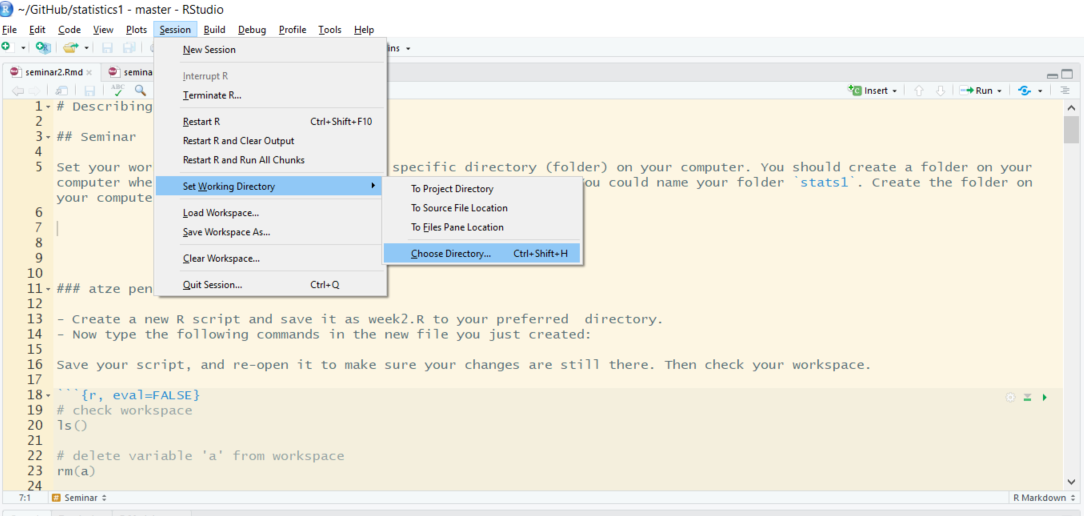
\includegraphics{./img/setwdir.png}

Create a new R script and save it as day1.R to your \texttt{Stats101} directory.

At the beginning of each new script, we want to clear the workspace. The workspace is stored in working memory on our computer. If we do not clear it for a new script, it becomes too full over time. Our computer will slow down and it will become difficult for us to know which objects are stored in working memory.

Again, as we are starting a new script we should check the contents of our workspace like so:

\begin{Shaded}
\begin{Highlighting}[]
\CommentTok{# check workspace}
\KeywordTok{ls}\NormalTok{()}
\end{Highlighting}
\end{Shaded}

Again to remove a specific object, we use the \texttt{rm()} function which stands for remove. Within the round brackets, we put the name of the object we want to remove. We could remove the object \texttt{a} like so:

\begin{Shaded}
\begin{Highlighting}[]
\CommentTok{# delete variable 'a' from workspace}
\KeywordTok{rm}\NormalTok{(a)}
\end{Highlighting}
\end{Shaded}

At the beginning of each script, we should always clear the entire workspace. We can do so in the following way:

\begin{Shaded}
\begin{Highlighting}[]
\CommentTok{# delete everything from workspace}
\KeywordTok{rm}\NormalTok{( }\DataTypeTok{list =} \KeywordTok{ls}\NormalTok{() )}
\end{Highlighting}
\end{Shaded}

You can also clear text from the console window. To do so press Crtl+l on Windows or Command+l on Mac.

\hypertarget{loading-data}{%
\subsubsection{Loading data}\label{loading-data}}

Data comes in different file formats such as \texttt{.txt}, \texttt{.csv}, \texttt{.xlsx}, \texttt{.RData}, \texttt{.dta} and many more. To know the file type of a file right click on it and view preferences (in Windows explorer or Mac finder).

R can load files coming in many different file formats. To find out how to import a file coming in a specific format, it is usually a good idea to the google ``R load file\_format''.

\hypertarget{importing-a-dataset-in-.csv-format}{%
\subsubsection{\texorpdfstring{Importing a dataset in \texttt{.csv} format}{Importing a dataset in .csv format}}\label{importing-a-dataset-in-.csv-format}}

One of the most common file types is \texttt{.csv} which means comma separated values. Columns are separated by commas and rows by line breaks.

Essentially, its best to work with this data format as it can be easily loaded into R, but also easy opening outside of R.

The dataset's name is ``non\_western\_immigrants.csv''. To load it, we use the \texttt{read.csv()} function.

\begin{Shaded}
\begin{Highlighting}[]
\NormalTok{dat1 <-}\StringTok{ }\KeywordTok{read.csv}\NormalTok{(}\StringTok{"non_western_immigrants.csv"}\NormalTok{)}
\end{Highlighting}
\end{Shaded}

\hypertarget{importing-a-dataset-in-excel-xlsx-format}{%
\subsubsection{Importing a dataset in Excel (xlsx) format}\label{importing-a-dataset-in-excel-xlsx-format}}

Another common file format is Microsoft's Excel \texttt{xlsx} format. We will load a dataset in this format now. To do so, we will need to install a package first. Packages are additional functions that we can add to R. A package is like an app on our phones.

We install the \texttt{readxl} package using \texttt{install.packages("readxl")}.

\begin{Shaded}
\begin{Highlighting}[]
\KeywordTok{install.packages}\NormalTok{(}\StringTok{"readxl"}\NormalTok{)}
\end{Highlighting}
\end{Shaded}

We only need to install a package once. It does not hurt to do it more often though, because every time we install, it will install the most recent version of the package.

Once a package is installed, we need to load it using the \texttt{library()} function.

\begin{Shaded}
\begin{Highlighting}[]
\KeywordTok{library}\NormalTok{(readxl)}
\end{Highlighting}
\end{Shaded}

To load the excel file, we can now use the \texttt{read\_excel()} function that is included in the \texttt{readxl} library. We need to provide the following arguments to the function:

\begin{longtable}[]{@{}ll@{}}
\toprule
Argument & Description\tabularnewline
\midrule
\endhead
path & Filename of excel sheet\tabularnewline
sheet & Sheet number to import\tabularnewline
\bottomrule
\end{longtable}

Now, let's load the file:

\begin{Shaded}
\begin{Highlighting}[]
\NormalTok{dat2 <-}\StringTok{ }\KeywordTok{read_excel}\NormalTok{(}\StringTok{"non_western_immigrants.xlsx"}\NormalTok{, }\DataTypeTok{sheet =} \DecValTok{1}\NormalTok{)}
\end{Highlighting}
\end{Shaded}

\hypertarget{importing-a-dataset-in-rdata-format}{%
\subsubsection{Importing a dataset in RData format}\label{importing-a-dataset-in-rdata-format}}

The native file format of R is called \texttt{.RData}. To load files saved in this format, we use the \texttt{load()} function like so:

\begin{Shaded}
\begin{Highlighting}[]
\KeywordTok{load}\NormalTok{(}\DataTypeTok{file =} \StringTok{"non_western_immigrants.RData"}\NormalTok{)}
\end{Highlighting}
\end{Shaded}

Notice that we usually need to assign the object we load to using the \texttt{\textless{}-} operator. The \texttt{load()} function is an exception where we do not need to do this.

\hypertarget{importing-a-dataset-in-.txt-format.}{%
\subsubsection{Importing a dataset in .txt format.}\label{importing-a-dataset-in-.txt-format.}}

Loading a dataset that comes in .txt format requires some additional information. The format is a text format and we need to know how the columns are separated. Usually it is enough to open the file in a word processor such as notepad to see how this is done. The most common ways to separate columns is by using commas or tabs but other separators such as for instance semicolons are sometimes also used.

In our example, columns are separated by semicolons. We use the \texttt{read.table()} function and provide the following arguments:

\begin{longtable}[]{@{}ll@{}}
\toprule
Argument & Description\tabularnewline
\midrule
\endhead
file & Filename of excel sheet\tabularnewline
sep & the symbol that separates columns\tabularnewline
header & whether the first row contains variable names or not\tabularnewline
\bottomrule
\end{longtable}

\begin{Shaded}
\begin{Highlighting}[]
\NormalTok{dat3 <-}\StringTok{ }\KeywordTok{read.table}\NormalTok{(}\DataTypeTok{file =} \StringTok{"non_western_immigrants.txt"}\NormalTok{, }\DataTypeTok{sep =}\StringTok{";"}\NormalTok{, }\DataTypeTok{header =} \OtherTok{TRUE}\NormalTok{)}
\end{Highlighting}
\end{Shaded}

\hypertarget{saving-data-frames}{%
\subsubsection{Saving data frames}\label{saving-data-frames}}

Datasets can be exported in many different file formats. We recommend exporting files as ``.csv'' files because csv is a very common file type. Such files can be handled by all statistical packages including Microsoft's Excel. We need to provide five arguments.

\begin{longtable}[]{@{}ll@{}}
\toprule
Argument & Description\tabularnewline
\midrule
\endhead
x & The name of the object\tabularnewline
file & The file name\tabularnewline
sep & The symbol that separates columns\tabularnewline
col.names & = TRUE saves the variable names (recommended)\tabularnewline
row.names & = FALSE omits the row names (recommended)\tabularnewline
\bottomrule
\end{longtable}

Lets save the data we have open on pereceptions of non-western immigration. It is important to select a new file name, i.e.~``newdata.csv'', otherwise R overwrites the original dataframe and data may be lost. If updating a dataframe, it is good practice to save a file as V1.0, then V1.1 and so on. Let's try this below:

\begin{Shaded}
\begin{Highlighting}[]
\KeywordTok{write.table}\NormalTok{(dat3, }
            \DataTypeTok{file =} \StringTok{"non_western_immigrants_V1.1.csv"}\NormalTok{,}
            \DataTypeTok{sep =} \StringTok{","}\NormalTok{,}
            \DataTypeTok{row.names =} \OtherTok{FALSE}\NormalTok{,}
            \DataTypeTok{col.names =} \OtherTok{TRUE}
\NormalTok{)}
\end{Highlighting}
\end{Shaded}

\hypertarget{descriptive-statistics}{%
\section{Descriptive Statistics}\label{descriptive-statistics}}

\hypertarget{seminar-3}{%
\subsection{Seminar}\label{seminar-3}}

Descriptive statistics are a good way to get a ``feel'' for the data and are an important first step for data analysis. Here we will explore two types: central tendency and dispersion.

Again, as good practice, let's first clear our workspace:

\begin{Shaded}
\begin{Highlighting}[]
\KeywordTok{rm}\NormalTok{( }\DataTypeTok{list =} \KeywordTok{ls}\NormalTok{() )}
\end{Highlighting}
\end{Shaded}

\hypertarget{central-tendency}{%
\subsubsection{Central tendency}\label{central-tendency}}

Central tendency explores the value of the observation at the center of a variable's distribution. This is the average or ``typical'' observation. What measure of central tendency you use depends on type of variable. In general, you use the following measures:

\begin{verbatim}
◦ Categorical variables – mode
◦ Ordinal variables - median
◦ Continuous variables – mean
\end{verbatim}

As a recap:

\begin{verbatim}
◦ Categorical variables are unranked categories, such as political parties.
◦ Ordinal variables have categories that are ranked on a scale, i.e. council tax bands.
◦ Continuous variables have integer values and are simply not countable, i.e.income.
◦ Count variables represent countable data such as crime incidents
◦ Binary variables have only two categories i.e. employed or unemployed.
\end{verbatim}

Let's first open some real data again:

\begin{Shaded}
\begin{Highlighting}[]
\NormalTok{dat1 <-}\StringTok{ }\KeywordTok{read.csv}\NormalTok{(}\StringTok{"non_western_immigrants.csv"}\NormalTok{, }\DataTypeTok{stringsAsFactors =} \OtherTok{FALSE}\NormalTok{)}
\KeywordTok{dim}\NormalTok{ (dat1)}
\end{Highlighting}
\end{Shaded}

\begin{verbatim}
[1] 1049   13
\end{verbatim}

We can explore this in R by summarising our data:
.

\begin{Shaded}
\begin{Highlighting}[]
\KeywordTok{summary}\NormalTok{( dat1)}
\end{Highlighting}
\end{Shaded}

\begin{verbatim}
    IMMBRIT       over.estimate         RSex            RAge      
 Min.   :  0.00   Min.   :0.0000   Min.   :1.000   Min.   :17.00  
 1st Qu.: 10.00   1st Qu.:0.0000   1st Qu.:1.000   1st Qu.:36.00  
 Median : 25.00   Median :1.0000   Median :2.000   Median :49.00  
 Mean   : 29.03   Mean   :0.7235   Mean   :1.544   Mean   :49.75  
 3rd Qu.: 40.00   3rd Qu.:1.0000   3rd Qu.:2.000   3rd Qu.:62.00  
 Max.   :100.00   Max.   :1.0000   Max.   :2.000   Max.   :99.00  
    Househld         paper          WWWhourspW        religious     
 Min.   :1.000   Min.   :0.0000   Min.   :  0.000   Min.   :0.0000  
 1st Qu.:1.000   1st Qu.:0.0000   1st Qu.:  0.000   1st Qu.:0.0000  
 Median :2.000   Median :0.0000   Median :  2.000   Median :0.0000  
 Mean   :2.392   Mean   :0.4538   Mean   :  5.251   Mean   :0.4929  
 3rd Qu.:3.000   3rd Qu.:1.0000   3rd Qu.:  7.000   3rd Qu.:1.0000  
 Max.   :8.000   Max.   :1.0000   Max.   :100.000   Max.   :1.0000  
  employMonths        urban        health.good        HHInc       
 Min.   :  1.00   Min.   :1.000   Min.   :0.000   Min.   : 1.000  
 1st Qu.: 72.00   1st Qu.:2.000   1st Qu.:2.000   1st Qu.: 6.000  
 Median : 72.00   Median :3.000   Median :2.000   Median : 9.000  
 Mean   : 86.56   Mean   :2.568   Mean   :2.044   Mean   : 9.586  
 3rd Qu.: 72.00   3rd Qu.:3.000   3rd Qu.:3.000   3rd Qu.:13.000  
 Max.   :600.00   Max.   :4.000   Max.   :3.000   Max.   :17.000  
   party_self   
 Min.   :1.000  
 1st Qu.:1.000  
 Median :2.000  
 Mean   :3.825  
 3rd Qu.:7.000  
 Max.   :7.000  
\end{verbatim}

However, this can be less useful when you have many variables in the data frame. So instead you can summzarise the variables of interest by subsetting:

\begin{Shaded}
\begin{Highlighting}[]
\KeywordTok{summary}\NormalTok{ (dat1[ , }\KeywordTok{c}\NormalTok{(}\StringTok{"IMMBRIT"}\NormalTok{, }\StringTok{"over.estimate"}\NormalTok{)])}
\end{Highlighting}
\end{Shaded}

\begin{verbatim}
    IMMBRIT       over.estimate   
 Min.   :  0.00   Min.   :0.0000  
 1st Qu.: 10.00   1st Qu.:0.0000  
 Median : 25.00   Median :1.0000  
 Mean   : 29.03   Mean   :0.7235  
 3rd Qu.: 40.00   3rd Qu.:1.0000  
 Max.   :100.00   Max.   :1.0000  
\end{verbatim}

Here the mean and median is reported. Again the median is relevant for ordinal values, while the mean is best for continuous, count and binary variables.

Large differences between the median and mean could indicate that a variable is skewed; when a variable has extreme values or many 0s which drags the mean either side of the median. For example, we often refer to ``median incomes,'' even though income is a continous variable. Here the median is used because the mean is dragged to the right by extremely wealthy outliers, while most incomes are in fact clustered as the lower end. The median income in the UK for 2014/15, before housing costs, was £473 per week. But for the mean, weekly income is placed at £581.

You may have noticed that the mode is not reported. To gain the mode you can create a frequency table and then use the order function to display the most common categories first. This is done by using the table and order functions:

\begin{Shaded}
\begin{Highlighting}[]
\NormalTok{a <-}\StringTok{ }\KeywordTok{table}\NormalTok{(dat1}\OperatorTok{$}\NormalTok{party_self)}
\NormalTok{a[}\KeywordTok{order}\NormalTok{(a, }\DataTypeTok{decreasing =} \OtherTok{TRUE}\NormalTok{)]}
\end{Highlighting}
\end{Shaded}

\begin{verbatim}

  7   1   2   6   5   4   3 
383 284 280  32  31  23  16 
\end{verbatim}

As you can see, category 7 is the most common category, with the number of observations reported below the category.

\hypertarget{dispersion}{%
\subsubsection{Dispersion}\label{dispersion}}

Dispersion measures the spread of values within a variable. Again, the precise measure of dispersion depends on the level of measurement:

\begin{verbatim}
◦ Categorical/binary variables – proportion of each category
◦ Ordinal variables – range or interquartile range
◦ Continuous/count variables – variance or the standard deviation
\end{verbatim}

\textbf{\emph{Categorical variables and proportional percentages}}

Let's first start with categorical variables (not this is also applicable for binary variables). Here we should again look at the a frequency table to understand the proportion of each category, in this case the proportion of observations for each political party:

\begin{Shaded}
\begin{Highlighting}[]
\CommentTok{#absolute frequency}
\NormalTok{table1 <-}\StringTok{ }\KeywordTok{table}\NormalTok{ (dat1}\OperatorTok{$}\NormalTok{party_self)}
\end{Highlighting}
\end{Shaded}

\begin{Shaded}
\begin{Highlighting}[]
\CommentTok{#and the percentages, rounded by two decimal spaces and then multiplied by 100}
\KeywordTok{round}\NormalTok{ (table1 }\OperatorTok{/}\KeywordTok{sum}\NormalTok{(table1), }\DecValTok{2}\NormalTok{)}\OperatorTok{*}\DecValTok{100}
\end{Highlighting}
\end{Shaded}

\begin{verbatim}

 1  2  3  4  5  6  7 
27 27  2  2  3  3 37 
\end{verbatim}

This variable does not have labels for the categories, but by looking at the codebook of this data set we know the categories are as followed:
1 - Conservatives
2 - Labour
3 - SNP
4 - Green
5 - UKIP
6 - BNP
7 - Other

Perhaps this is not the best sample of our population, since there is no category for the Liberal Democrats!

\textbf{\emph{Ordinal variables and the interquartile range}}

For ordinal variables, the most useful way to explore dispersion is by looking at the interquartile range. This can be visualised by plotting a simple box plot.

Note that with plots in R we have to provide arguments to design the plot, which are seperated by commas. Below we select:
i) the variable of interest within the data frame (using the \$ symbol),
ii) add labels for the graph and y-axis,
iii) remove the frame around the plot using the frame.plot function
iv) choose the colour.

\begin{Shaded}
\begin{Highlighting}[]
\KeywordTok{boxplot}\NormalTok{(}
\NormalTok{  dat1}\OperatorTok{$}\NormalTok{HHInc, }
  \DataTypeTok{main =} \StringTok{"Income in the UK"}\NormalTok{,}
  \DataTypeTok{ylab =} \StringTok{"Income Index"}\NormalTok{, }
  \DataTypeTok{frame.plot =} \OtherTok{FALSE}\NormalTok{, }
  \DataTypeTok{col =} \StringTok{"darkgray"}
\NormalTok{)}
\end{Highlighting}
\end{Shaded}

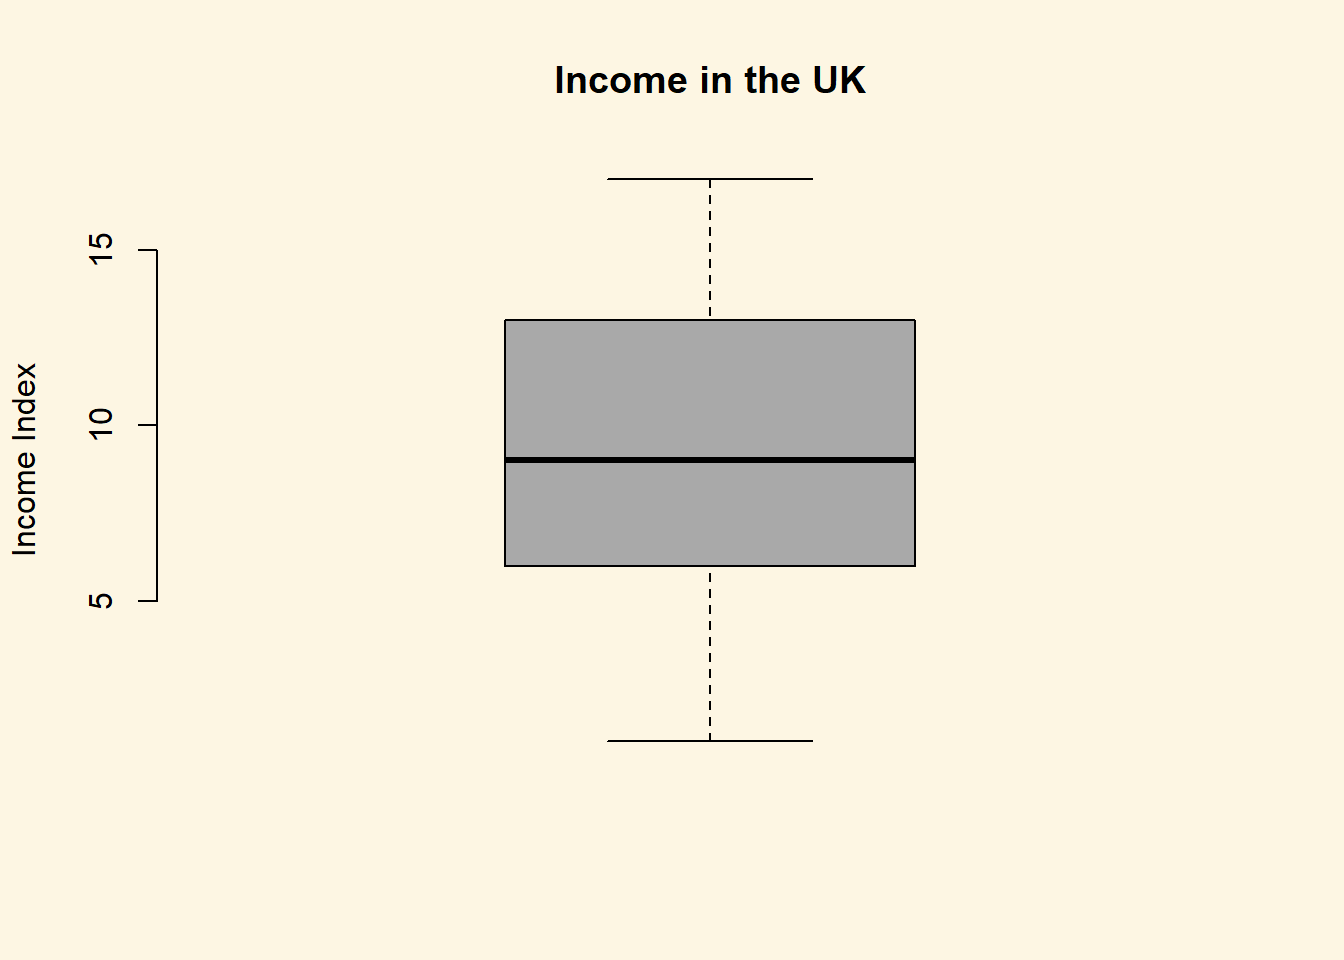
\includegraphics{stats101_files/figure-latex/unnamed-chunk-63-1.pdf}

The box that is displayed within the plot represents the location of 50\% of the data, between the 25\% and 75\% quartiles. The line within the box tells us the median. The two lines outside of the box shows us the data that falls within 1.5 times the quartiles.

\textbf{\emph{Continuous variables and the standard deviation}}

For continuous (and count) variables we can look at the standard deviation. This tells us where 68\% of the data can be found, since 68\% of the data falls within one standard deviation of the mean. This can be done in R with a simple function. Here we are looking at British perceptions of non-Western immigration:

\begin{Shaded}
\begin{Highlighting}[]
\KeywordTok{sd}\NormalTok{(dat1}\OperatorTok{$}\NormalTok{IMMBRIT)}
\end{Highlighting}
\end{Shaded}

\begin{verbatim}
[1] 21.06331
\end{verbatim}

We can then compare this to the mean, which is another way to see if a continous variable is skewed:

\begin{Shaded}
\begin{Highlighting}[]
\KeywordTok{mean}\NormalTok{(dat1}\OperatorTok{$}\NormalTok{IMMBRIT)}
\end{Highlighting}
\end{Shaded}

\begin{verbatim}
[1] 29.03051
\end{verbatim}

With the standard deviation at 21 and the mean at 29, we can see there is a large gap which indicates skewedness. But we can also simply visualise this by plotting the density of the variable:

\begin{Shaded}
\begin{Highlighting}[]
\KeywordTok{plot}\NormalTok{(}\KeywordTok{density}\NormalTok{(dat1}\OperatorTok{$}\NormalTok{IMMBRIT))}
\end{Highlighting}
\end{Shaded}

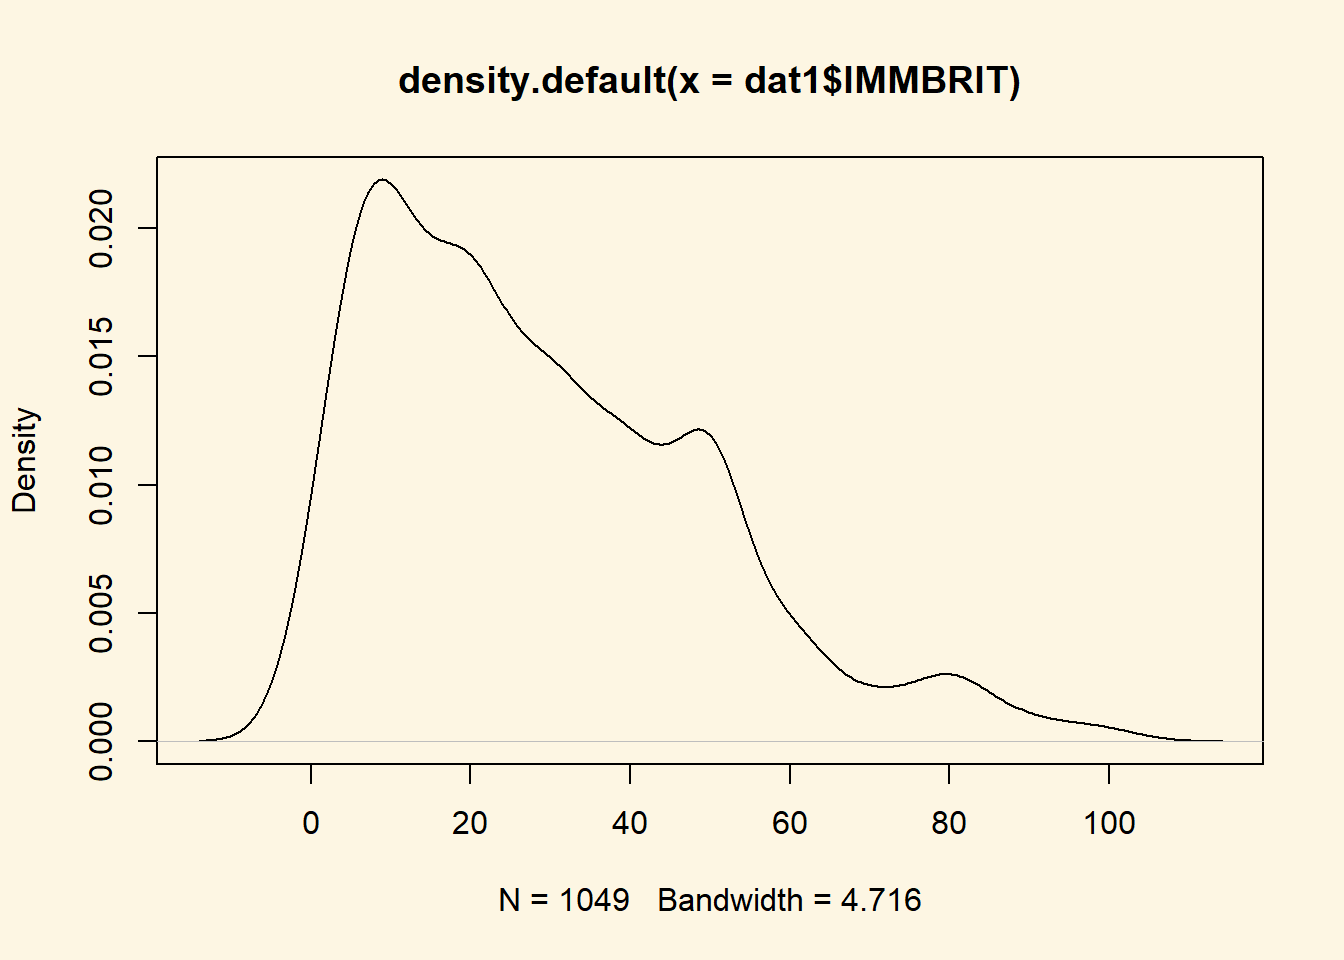
\includegraphics{stats101_files/figure-latex/unnamed-chunk-66-1.pdf}

As we can see most of the data is in the left hand side of the graph with fewer larger values on the far right of the graph. This drags the mean to the right which explains the large difference with the standard deviation. In this case it would be more appropriate to use the median (as is the case with income in the example above). When we run the median below, it is much closer to the centre of the data:

\begin{Shaded}
\begin{Highlighting}[]
\KeywordTok{median}\NormalTok{(dat1}\OperatorTok{$}\NormalTok{IMMBRIT)}
\end{Highlighting}
\end{Shaded}

\begin{verbatim}
[1] 25
\end{verbatim}

To clear the graphs from our workspace, we can use the dev.off function with brackets:

\begin{Shaded}
\begin{Highlighting}[]
\KeywordTok{dev.off}\NormalTok{()}
\end{Highlighting}
\end{Shaded}

\begin{verbatim}
null device 
          1 
\end{verbatim}

\hypertarget{correlations-and-differences-in-means}{%
\section{Correlations and differences in means}\label{correlations-and-differences-in-means}}

\hypertarget{seminar-4}{%
\subsection{Seminar}\label{seminar-4}}

In this session, we will cover bivariate relationships, that is relationships between two variables. For relationships between two continuous variables, we will look at correlations and plots and for relationships between a continuous dependent variable and a binary independent variable, we will look at differences in means.

\hypertarget{bivariate-relationships}{%
\subsubsection{Bivariate relationships}\label{bivariate-relationships}}

In data analysis we are mostly interested in understanding the relationships between two (or more) variables. For instance, between a predictor (independent variable) and an outcome of interest (dependent variable). Summary statistics are often the first steps in trying to understand relationships between variables.

Initially we might want to visualise a relationship between an independent variable and a dependent variable (outcome). For example, we might want to see how two categories are related to an outcome of interest.

Again, as good practice, let's first clear our workspace before we start:

\begin{Shaded}
\begin{Highlighting}[]
\KeywordTok{rm}\NormalTok{( }\DataTypeTok{list =} \KeywordTok{ls}\NormalTok{() )}
\end{Highlighting}
\end{Shaded}

Let's open the data again:

\begin{Shaded}
\begin{Highlighting}[]
\NormalTok{dat1 <-}\StringTok{ }\KeywordTok{read.csv}\NormalTok{(}\StringTok{"non_western_immigrants.csv"}\NormalTok{, }\DataTypeTok{stringsAsFactors =} \OtherTok{FALSE}\NormalTok{)}
\KeywordTok{dim}\NormalTok{ (dat1)}
\end{Highlighting}
\end{Shaded}

\begin{verbatim}
[1] 1049   13
\end{verbatim}

Here we will compare if there are differences in perceptions of non-Western immigrants between those that identify with the Convervatives and those that support the Labour party.

We need to first create two new dummy variables from the categorical variable that lists identified political parties. These two binary variables will tell us observations where someone identifies with the Conservatives (1=yes and 0 = no) and the same for the Labour party (1=yes and 0=no). Here we have to use the ifelse function:

\begin{Shaded}
\begin{Highlighting}[]
\NormalTok{dat1}\OperatorTok{$}\NormalTok{conservatives <-}\StringTok{ }\KeywordTok{ifelse}\NormalTok{(dat1}\OperatorTok{$}\NormalTok{party_self }\OperatorTok{==}\StringTok{ }\DecValTok{1}\NormalTok{, }\DataTypeTok{yes =} \DecValTok{1}\NormalTok{, }\DataTypeTok{no =} \DecValTok{0}\NormalTok{)}
\NormalTok{dat1}\OperatorTok{$}\NormalTok{labour <-}\StringTok{ }\KeywordTok{ifelse}\NormalTok{(dat1}\OperatorTok{$}\NormalTok{party_self }\OperatorTok{==}\StringTok{ }\DecValTok{2}\NormalTok{, }\DataTypeTok{yes =} \DecValTok{1}\NormalTok{, }\DataTypeTok{no =} \DecValTok{0}\NormalTok{)}
\end{Highlighting}
\end{Shaded}

So we create new variables within our dataframe using categories from the party\_self variable. == 1 is the category we are choosing. If the ifelse statement is true, they do identify with that party, we code yes as a 1 and no as a 0.

We can now run plots for the Conservatives and Labour party. We need to select the arguments as before, including appropriate colours for the parties. Here we also set the ylim to show a scale of the data from 0-100. First for the Conservative party and then for the Labour party:

\begin{Shaded}
\begin{Highlighting}[]
\CommentTok{# separte plot window into 1 row and 2 columns}
\KeywordTok{par}\NormalTok{(}\DataTypeTok{mfrow=}\KeywordTok{c}\NormalTok{(}\DecValTok{1}\NormalTok{,}\DecValTok{2}\NormalTok{))}

\KeywordTok{boxplot}\NormalTok{(}
\NormalTok{  dat1}\OperatorTok{$}\NormalTok{IMMBRIT[dat1}\OperatorTok{$}\NormalTok{conservatives}\OperatorTok{==}\DecValTok{1}\NormalTok{],}
  \DataTypeTok{frame.plot =} \OtherTok{FALSE}\NormalTok{,}
  \DataTypeTok{xlab =} \StringTok{"Conservatives"}\NormalTok{,}
  \DataTypeTok{ylim =} \KeywordTok{c}\NormalTok{(}\DecValTok{0}\NormalTok{, }\DecValTok{100}\NormalTok{),}
  \DataTypeTok{col =} \StringTok{"blue"}
\NormalTok{)}

\KeywordTok{boxplot}\NormalTok{(}
\NormalTok{  dat1}\OperatorTok{$}\NormalTok{IMMBRIT[dat1}\OperatorTok{$}\NormalTok{labour}\OperatorTok{==}\DecValTok{1}\NormalTok{],}
  \DataTypeTok{frame.plot =} \OtherTok{FALSE}\NormalTok{,}
  \DataTypeTok{xlab =} \StringTok{"Labour"}\NormalTok{,}
  \DataTypeTok{ylim =} \KeywordTok{c}\NormalTok{(}\DecValTok{0}\NormalTok{, }\DecValTok{100}\NormalTok{),}
  \DataTypeTok{col =} \StringTok{"red"}
\NormalTok{)}
\end{Highlighting}
\end{Shaded}

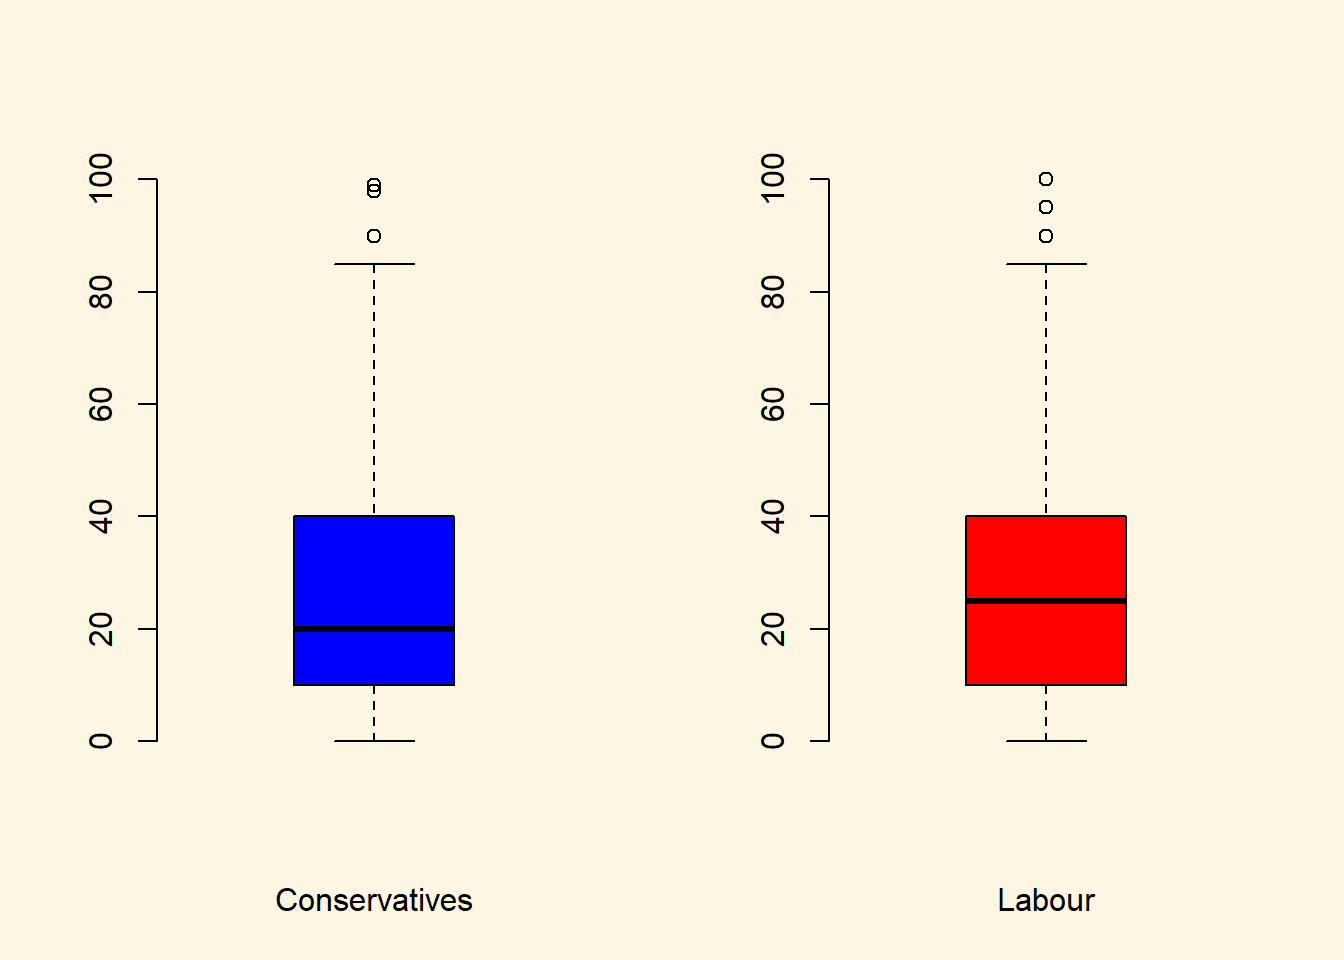
\includegraphics{stats101_files/figure-latex/unnamed-chunk-74-1.pdf}

Note: If you want to reset the plot window to one row and 1 column you need to run \texttt{par(mfrow=c(1,1)}.

Overall, there appears to be very little difference between the Conservatives and Labour distributions in regards to perceptions of non-Western immigrants. The dots at the top of the scale represent outlier cases, where perceptions overestimate the number of immigrants.

The higher values for the Labour party could be due to high Labour support in diverse urban centres such as London. Yet, these are just samples and a snapshot of the possible relationship.Samples are never the same and vary. For instance, crime is not statistic and will vary over time and space.

Can we be sure that this result did not simply occur by chance?

This brings us to the importance of hypothesis testing.

\hypertarget{hypothesis-testing}{%
\subsubsection{Hypothesis testing}\label{hypothesis-testing}}

Because relationships can occur by chance, hypotheis testing is central to statistics. The first step is to form our own hypothesis about a potential relationship between variables and then compare this against what is known as the null hypothesis. The null hypothesis represents the notion that nothing special has occured and that the relationship we are observing has only occured by chance, i.e.~getting heads when flipping a coin.

In the lecture slides, we cover this by exploring the Lady Tea Tasting Test (Fisher, 1925). When running statistics in R and other statistical packages, most models report a t-statistic and p-value, which we then informs us of whether we should reject the null hypothesis.

The t-statistic is easy to interpret. While we know 1 standard deviation from the mean represents 68\% of the distribution, more than 1.96 deviations is more than 95\% of the distribution. Therefore, if the t-statistic is higher than an absolute value of 1.96 (either 1.96 or -1.96), then the estimate we observe falls outside 95\% of possible resampled estimations and is simply too rare to have occured by chance.

The p-value is based on the t-statistic and provides the actually probability that a estimate occured by chance.
In most fields of research, the conventional threshold for a p-value is less than 0.05.This implies we will incorrectly reject the null hypothesis less than 5\% of the time.
A p-value of 0.01 implies we will incorrectly reject the null hypothesis 1\% of the time. So the lower the p-value, the more confidence we can have in our estimate.
If we reject the null hypothesis then the relationship we observe is statistically significant.

Let's move on to a t-test to assess and outcome and whether two categories are statistically significant from one another. Here we explore difference between two estimated means.

\hypertarget{t-test-difference-in-means}{%
\subsubsection{T-test (difference in means)}\label{t-test-difference-in-means}}

We are interested in whether there is a difference in income between countries that have an history of colonialisation and those that do not. Put more formally, we are interested in the difference between two conditional means. Recall that a conditional mean is the mean in a subpopulation, such as the mean of income given that the country was a victim of colonialisation (conditional mean 1).

The t-test is the appropriate test-statistic. Our interval-level dependent variable is \texttt{wdi\_gdpc} which is GDP per capita taken from the World Development Indicators of the World Bank. Our binary independent variable is \texttt{h\_j}.

Let's check the summary statistics of our dependent variable GDP per captia using the \href{https://www.rdocumentation.org/packages/base/versions/3.4.1/topics/summary}{\texttt{summary()}}. It returns several descriptive statistics as well as the number of NA observations (missing values). Missing values mean that we have no information on the correct value of the variable for an observation. Missing values may be missing for many different reasons. We need to be aware of missings because we cannot calculate with missings.

Lets bring the data in:{]}

\begin{Shaded}
\begin{Highlighting}[]
\NormalTok{dat2 <-}\StringTok{ }\KeywordTok{read.csv}\NormalTok{(}\StringTok{"QoG2012.csv"}\NormalTok{, }\DataTypeTok{stringsAsFactors =} \OtherTok{FALSE}\NormalTok{)}
\end{Highlighting}
\end{Shaded}

\begin{Shaded}
\begin{Highlighting}[]
\KeywordTok{summary}\NormalTok{(dat2}\OperatorTok{$}\NormalTok{wdi_gdpc)}
\end{Highlighting}
\end{Shaded}

\begin{verbatim}
   Min. 1st Qu.  Median    Mean 3rd Qu.    Max.    NA's 
  226.2  1768.0  5326.1 10184.1 12976.5 63686.7      16 
\end{verbatim}

We use the \texttt{which()} function to identify the row-numbers of the countries in our dataset that have a colonial history. The code below returns the row index numbers of countries with a history of colonialisation.

\begin{Shaded}
\begin{Highlighting}[]
\KeywordTok{which}\NormalTok{(dat2}\OperatorTok{$}\NormalTok{former_col }\OperatorTok{==}\StringTok{ }\DecValTok{1}\NormalTok{)}
\end{Highlighting}
\end{Shaded}

\begin{verbatim}
  [1]   3   5   6   8  11  12  13  15  17  18  20  21  22  23  24  26  27
 [18]  29  30  32  33  34  35  36  39  40  41  42  43  45  46  48  50  51
 [35]  52  53  54  56  58  61  62  64  66  67  69  70  71  72  73  74  77
 [52]  78  80  84  85  88  89  92  94  95  96  99 103 104 105 106 107 109
 [69] 110 111 116 117 118 119 120 123 125 126 127 129 130 131 132 133 134
 [86] 135 136 137 140 142 145 146 147 148 150 152 154 155 156 158 160 161
[103] 162 164 165 166 169 172 173 174 175 176 179 180 183 185 187 188 190
[120] 191 192 194
\end{verbatim}

Now, we can explore conditional means. Below we access the variable that we want (\texttt{wdi\_gdpc}) with the dollar sign and the rows in square brackets. The code below returns the per capita wealth of the countries with a colonial history:

\begin{Shaded}
\begin{Highlighting}[]
\KeywordTok{mean}\NormalTok{( dat2}\OperatorTok{$}\NormalTok{wdi_gdpc[dat2}\OperatorTok{$}\NormalTok{former_col }\OperatorTok{==}\StringTok{ }\DecValTok{1}\NormalTok{], }\DataTypeTok{na.rm =} \OtherTok{TRUE}\NormalTok{)}
\end{Highlighting}
\end{Shaded}

\begin{verbatim}
[1] 6599.714
\end{verbatim}

Now, go ahead and find the mean per capita wealth of countries without a colonial history:

\begin{Shaded}
\begin{Highlighting}[]
\KeywordTok{mean}\NormalTok{( dat2}\OperatorTok{$}\NormalTok{wdi_gdpc[dat2}\OperatorTok{$}\NormalTok{former_col }\OperatorTok{==}\StringTok{ }\DecValTok{0}\NormalTok{], }\DataTypeTok{na.rm =} \OtherTok{TRUE}\NormalTok{)}
\end{Highlighting}
\end{Shaded}

\begin{verbatim}
[1] 16415.39
\end{verbatim}

There is a clear numeric difference. Countries with a colonial history do appear to be significantly poorer.

However, we know that samples are subject to sampling variability. We therefore need to quantify the uncertainty that results from variable samples. To assess whether we can be reasonably sure that the difference between the estimates of wealth is not due to a strange sample or by chance, we carry out the t test to assess if there is a statistically significant difference between these populations:

\begin{Shaded}
\begin{Highlighting}[]
\KeywordTok{t.test}\NormalTok{(dat2}\OperatorTok{$}\NormalTok{wdi_gdpc[dat2}\OperatorTok{$}\NormalTok{former_col }\OperatorTok{==}\StringTok{ }\DecValTok{1}\NormalTok{], dat2}\OperatorTok{$}\NormalTok{wdi_gdpc[dat2}\OperatorTok{$}\NormalTok{former_col }\OperatorTok{==}\StringTok{ }\DecValTok{0}\NormalTok{],}
       \DataTypeTok{mu =} \DecValTok{0}\NormalTok{, }\DataTypeTok{alt =} \StringTok{"two.sided"}\NormalTok{, }\DataTypeTok{conf =} \FloatTok{0.95}\NormalTok{)}
\end{Highlighting}
\end{Shaded}

\begin{verbatim}

    Welch Two Sample t-test

data:  dat2$wdi_gdpc[dat2$former_col == 1] and dat2$wdi_gdpc[dat2$former_col == 0]
t = -5.0603, df = 101.69, p-value = 1.866e-06
alternative hypothesis: true difference in means is not equal to 0
95 percent confidence interval:
 -13663.313  -5968.043
sample estimates:
mean of x mean of y 
 6599.714 16415.392 
\end{verbatim}

Let's interpret the results we get from \texttt{t.test()}. In our example the question is: Do countries with a former colonial history have different mean income levels than countries without colonial history?

The dependent variable is income, while the indepedent variable is where a country has a colonial history.

We know that when the t-statistic is greater then 1.96 or than -1.96, then we can safely reject the null hypothesis, i.e.~it is less than 5\% likely the estimate occured by chance. The p-value gives us a more direct probability of us wrongly rejecting the null hypothesis of \texttt{1.866e-06}which means a p-value of \texttt{0.000001866}!!!

In the next line you see the 95\% confidence interval because we specified \texttt{conf=0.95}. If you were to take 100 samples and in each you checked the means of the two groups, 95 times the difference in means would be within the interval you see there.

At the very bottom you see the means of the dependent variable by the two groups of the independent variable. These are the conditional means that we estimated above. By minusing the \$6599.7 from \$16414.4, we know that former colonial countries are on average \$9814.70 worst off!

\hypertarget{relationships-between-continuous-variables}{%
\subsubsection{Relationships between continuous variables}\label{relationships-between-continuous-variables}}

One way to explore the relationship between two continous variables is to use correlation. This is a widely used as a summary statistic. Correlation is a measure of \textbf{linear} association. It can take values between -1 and +1. Where -1 is a perfect negative relationship, 0 is a no relationship and +1 is a perfect positive relationship. 0 means there is no relationship, as would be expected if the null hypothesis was true.

We estimate the correlation coefficient in the following:

\begin{Shaded}
\begin{Highlighting}[]
\KeywordTok{cor}\NormalTok{(}\DataTypeTok{y =}\NormalTok{ dat2}\OperatorTok{$}\NormalTok{undp_hdi, }\DataTypeTok{x =}\NormalTok{ dat2}\OperatorTok{$}\NormalTok{wbgi_cce, }\DataTypeTok{use =} \StringTok{"complete.obs"}\NormalTok{)}
\end{Highlighting}
\end{Shaded}

\begin{verbatim}
[1] 0.6821114
\end{verbatim}

\begin{longtable}[]{@{}ll@{}}
\toprule
\begin{minipage}[b]{0.11\columnwidth}\raggedright
Argument\strut
\end{minipage} & \begin{minipage}[b]{0.83\columnwidth}\raggedright
Description\strut
\end{minipage}\tabularnewline
\midrule
\endhead
\begin{minipage}[t]{0.11\columnwidth}\raggedright
\texttt{x}\strut
\end{minipage} & \begin{minipage}[t]{0.83\columnwidth}\raggedright
The independent variable that you want to correlate.\strut
\end{minipage}\tabularnewline
\begin{minipage}[t]{0.11\columnwidth}\raggedright
\texttt{y}\strut
\end{minipage} & \begin{minipage}[t]{0.83\columnwidth}\raggedright
The dependent variable that you want to correlate.\strut
\end{minipage}\tabularnewline
\begin{minipage}[t]{0.11\columnwidth}\raggedright
\texttt{use}\strut
\end{minipage} & \begin{minipage}[t]{0.83\columnwidth}\raggedright
How R should handle missing values. \texttt{use="complete.obs"} will use only those rows where neither \texttt{x} nor \texttt{y} is missing.\strut
\end{minipage}\tabularnewline
\bottomrule
\end{longtable}

The interpretation of the correlation coefficient is that there is a positive relationship. However, the correlation coefficients does not tell us the magnitude of the relationship.

Another weakness is that it is a measure of linear association only. That means, there could be a curvilinear (or non-linear) realtionship which we miss (for instance a u-shaped relationship).

Often the best way to get a sense for the relationship beetween two continuous variables is visual inspection using a scatter plot. The human development index measures the quality of life and the World Bank Control of Corruption Index is a measure for the quality if institutions. We want to evaluate whether the two variables are related at all. Here, we could form the hypothesis that better insitutions improve the quality of life of citizens.

To investigate this relationship, we construct a scatterplot.

\begin{Shaded}
\begin{Highlighting}[]
\KeywordTok{plot}\NormalTok{(}
  \DataTypeTok{x =}\NormalTok{ dat2}\OperatorTok{$}\NormalTok{wbgi_cce,}
  \DataTypeTok{y =}\NormalTok{ dat2}\OperatorTok{$}\NormalTok{undp_hdi,}
  \DataTypeTok{xlim =} \KeywordTok{c}\NormalTok{(}\OperatorTok{-}\DecValTok{2}\NormalTok{, }\DecValTok{3}\NormalTok{),}
  \DataTypeTok{ylim =} \KeywordTok{c}\NormalTok{(}\DecValTok{0}\NormalTok{, }\DecValTok{1}\NormalTok{),}
  \DataTypeTok{frame =} \OtherTok{FALSE}\NormalTok{,}
  \DataTypeTok{xlab =} \StringTok{"World Bank Control of Corruption Index"}\NormalTok{,}
  \DataTypeTok{ylab =} \StringTok{"UNDP Human Development Index"}\NormalTok{,}
  \DataTypeTok{main =} \StringTok{"Relationship b/w Quality of Institutions and Quality of Life"}\NormalTok{,}
  \DataTypeTok{pch =} \DecValTok{16}\NormalTok{,}
  \DataTypeTok{col =} \StringTok{"darkgray"}
\NormalTok{)}
\end{Highlighting}
\end{Shaded}

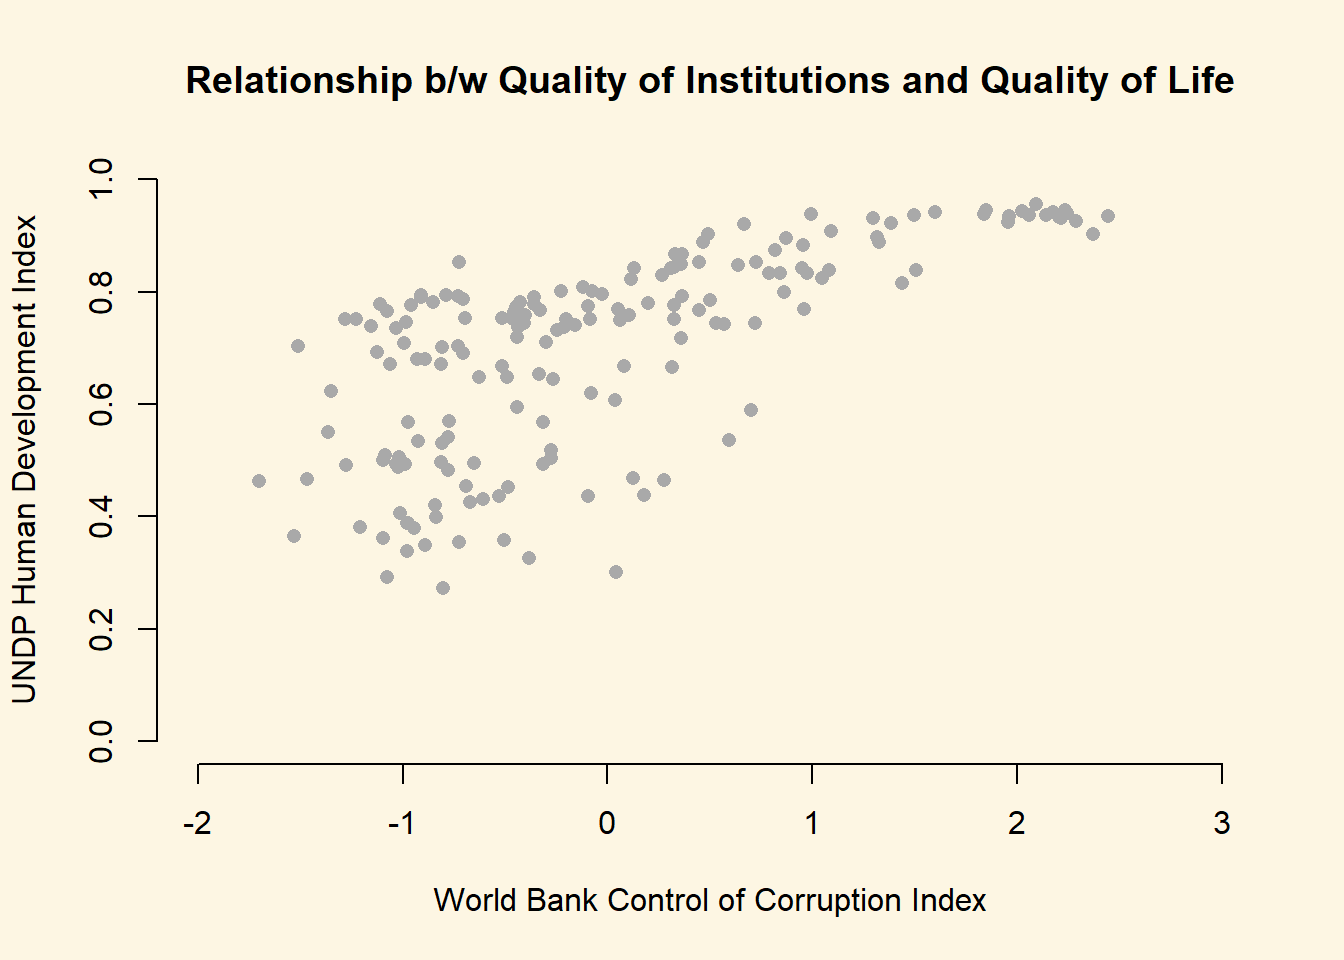
\includegraphics{stats101_files/figure-latex/unnamed-chunk-83-1.pdf}

The plot will give you a good idea whether about whether these two variables are related or not. Sometimes, the correleation coefficient is reported.

Overall, summary statistics are an important step in understanding the relationship between variables and whether such relationships occur by chance. However, this does not tell us much about the magnitude of the relationships we seek to explore. For this we must switch our attention to linear regression, which provides coefficients that can be interpreted as the extent to which a independent variable impacts a dependent variable. Linear regression also allows us to control for other independent variables which may also explain our dependent variable, i.e.~alternative explainations of the outcome we are exploring.

\hypertarget{regression}{%
\section{Regression}\label{regression}}

\hypertarget{seminar-5}{%
\subsection{Seminar}\label{seminar-5}}

In this section, we will cover regression models. We will first introduce the bivariate linear regression model. We will then move to linear models with multiple independent variables.

\hypertarget{bivariate-linear-regression}{%
\subsubsection{Bivariate linear regression}\label{bivariate-linear-regression}}

We will use a dataset collected by the US census bureau that contains several socioeconomic indicators.

\begin{Shaded}
\begin{Highlighting}[]
\NormalTok{communities <-}\StringTok{ }\KeywordTok{read.csv}\NormalTok{(}\StringTok{"communities.csv"}\NormalTok{)}
\end{Highlighting}
\end{Shaded}

The dataset includes 38 variables but we're only interested in a handful at the moment.

\begin{tabular}{l|l}
\hline
Variable & Description\\
\hline
PctUnemployed & proportion of citizens in each community who are unemployed\\
\hline
PctNotHSGrad & proportion of citizens in each community who failed to finish high-school\\
\hline
population & proportion of adult population living in cities\\
\hline
\end{tabular}

If we summarize these variables with the \texttt{summary()} function, we will see that they are both measured as proportions (they vary between 0 and 1):

\begin{Shaded}
\begin{Highlighting}[]
\KeywordTok{summary}\NormalTok{(communities}\OperatorTok{$}\NormalTok{PctUnemployed)}
\end{Highlighting}
\end{Shaded}

\begin{verbatim}
   Min. 1st Qu.  Median    Mean 3rd Qu.    Max. 
 0.0000  0.2200  0.3200  0.3635  0.4800  1.0000 
\end{verbatim}

\begin{Shaded}
\begin{Highlighting}[]
\KeywordTok{summary}\NormalTok{(communities}\OperatorTok{$}\NormalTok{PctNotHSGrad)}
\end{Highlighting}
\end{Shaded}

\begin{verbatim}
   Min. 1st Qu.  Median    Mean 3rd Qu.    Max. 
 0.0000  0.2300  0.3600  0.3833  0.5100  1.0000 
\end{verbatim}

It will be a little easier to interpret the regression output if we convert these to percentages rather than proportions. We can do this with the following lines of code:

\begin{Shaded}
\begin{Highlighting}[]
\NormalTok{communities}\OperatorTok{$}\NormalTok{PctUnemployed <-}\StringTok{ }\NormalTok{communities}\OperatorTok{$}\NormalTok{PctUnemployed }\OperatorTok{*}\StringTok{ }\DecValTok{100}
\NormalTok{communities}\OperatorTok{$}\NormalTok{PctNotHSGrad <-}\StringTok{ }\NormalTok{communities}\OperatorTok{$}\NormalTok{PctNotHSGrad }\OperatorTok{*}\StringTok{ }\DecValTok{100}
\end{Highlighting}
\end{Shaded}

We can begin by drawing a scatterplot with the percentage of unemployed people on the y-axis and the percentage of adults without high-school education on the x-axis.

\begin{Shaded}
\begin{Highlighting}[]
\KeywordTok{plot}\NormalTok{(}
  \DataTypeTok{x =}\NormalTok{ communities}\OperatorTok{$}\NormalTok{PctNotHSGrad,}
  \DataTypeTok{y =}\NormalTok{ communities}\OperatorTok{$}\NormalTok{PctUnemployed,}
  \DataTypeTok{xlab =} \StringTok{"Adults without high school education (%)"}\NormalTok{,}
  \DataTypeTok{ylab =} \StringTok{"Unemployment (%)"}\NormalTok{,}
  \DataTypeTok{frame.plot =} \OtherTok{FALSE}\NormalTok{,}
  \DataTypeTok{pch =} \DecValTok{20}\NormalTok{,}
  \DataTypeTok{col =} \StringTok{"LightSkyBlue"}
\NormalTok{)}
\end{Highlighting}
\end{Shaded}

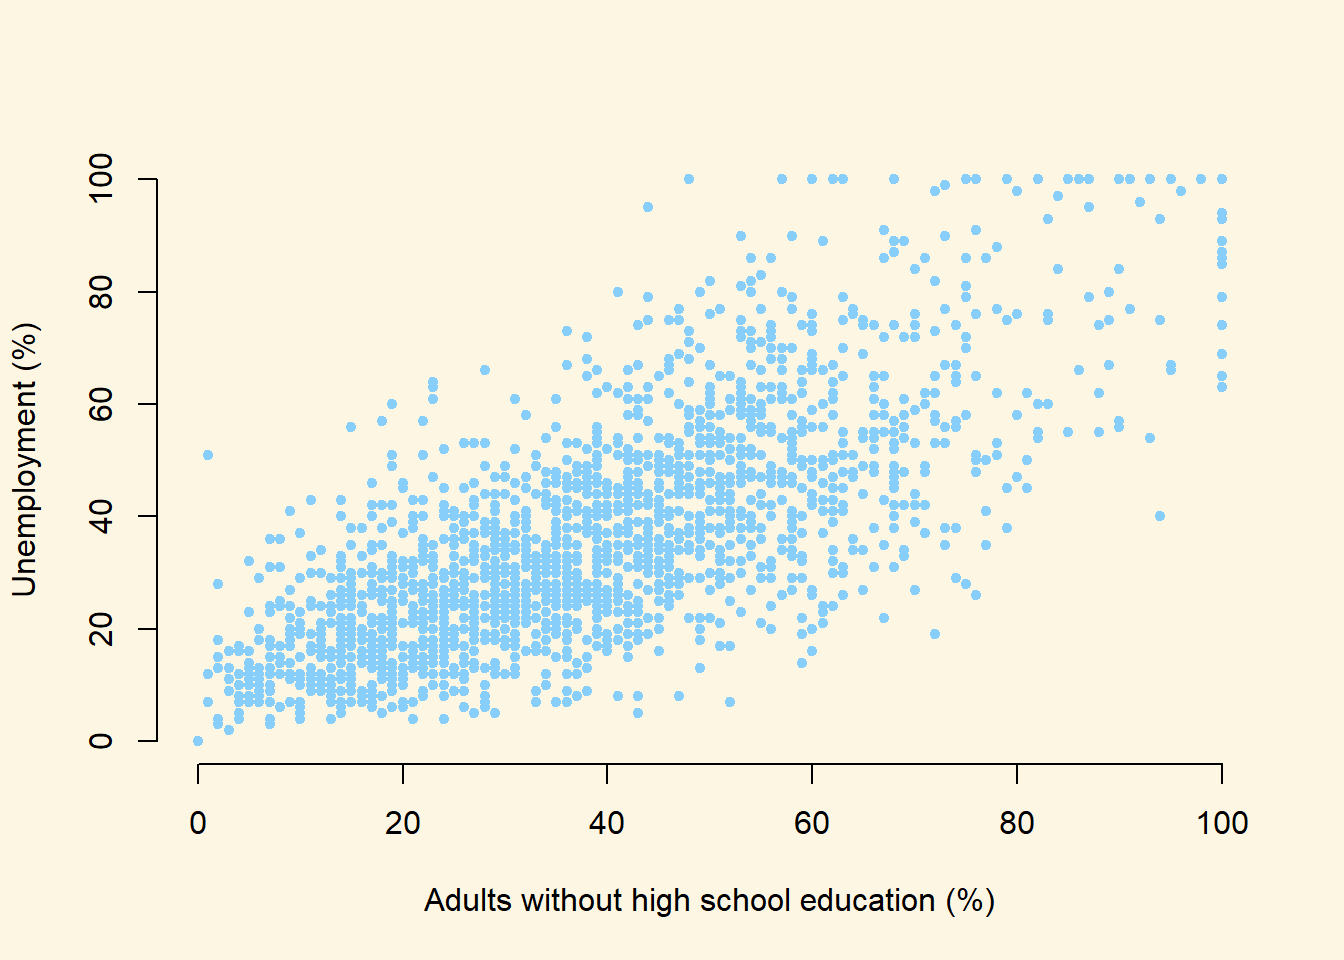
\includegraphics{stats101_files/figure-latex/unnamed-chunk-90-1.pdf}

From looking at the plot, what is the association between the unemployment rate and lack of high-school level education?

In order to answer that question empirically, we will run a linear regression using the \href{http://bit.ly/R_lm}{\texttt{lm()}} function in R. The \href{http://bit.ly/R_lm}{\texttt{lm()}} function needs to know a) the relationship we're trying to model and b) the dataset for our observations. The two arguments we need to provide to the \href{http://bit.ly/R_lm}{\texttt{lm()}} function are described below.

\begin{longtable}[]{@{}ll@{}}
\toprule
\begin{minipage}[b]{0.11\columnwidth}\raggedright
Argument\strut
\end{minipage} & \begin{minipage}[b]{0.83\columnwidth}\raggedright
Description\strut
\end{minipage}\tabularnewline
\midrule
\endhead
\begin{minipage}[t]{0.11\columnwidth}\raggedright
\texttt{formula}\strut
\end{minipage} & \begin{minipage}[t]{0.83\columnwidth}\raggedright
The \texttt{formula} describes the relationship between the dependent and independent variables, for example \texttt{dependent.variable\ \textasciitilde{}\ independent.variable} In our case, we'd like to model the relationship using the formula: \texttt{PctUnemployed\ \textasciitilde{}\ PctNotHSGrad}\strut
\end{minipage}\tabularnewline
\begin{minipage}[t]{0.11\columnwidth}\raggedright
\texttt{data}\strut
\end{minipage} & \begin{minipage}[t]{0.83\columnwidth}\raggedright
This is simply the name of the dataset that contains the variable of interest. In our case, this is the merged dataset called \texttt{communities}.\strut
\end{minipage}\tabularnewline
\bottomrule
\end{longtable}

For more information on how the \texttt{lm()} function works, type help(lm) in R.

\begin{Shaded}
\begin{Highlighting}[]
\NormalTok{model1 <-}\StringTok{ }\KeywordTok{lm}\NormalTok{(PctUnemployed }\OperatorTok{~}\StringTok{ }\NormalTok{PctNotHSGrad, }\DataTypeTok{data =}\NormalTok{ communities)}
\end{Highlighting}
\end{Shaded}

\hypertarget{interpreting-regression-output}{%
\subsubsection{Interpreting Regression Output}\label{interpreting-regression-output}}

The \href{http://bit.ly/R_lm}{\texttt{lm()}} function has modeled the relationship between \texttt{PctUnemployed} and \texttt{PctNotHSGrad} and we've saved it in an object called \texttt{model1}. Let's use the \href{http://bit.ly/R_summary}{\texttt{summary()}} function to see what this linear model looks like.

\begin{Shaded}
\begin{Highlighting}[]
\KeywordTok{summary}\NormalTok{(model1)}
\end{Highlighting}
\end{Shaded}

The output from \href{http://bit.ly/R_summary}{\texttt{summary()}} might seem overwhelming at first so let's break it down one item at a time.

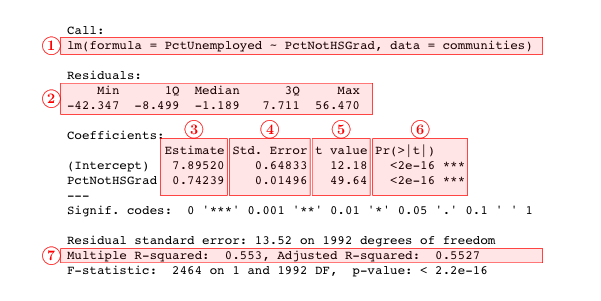
\includegraphics[width=7.29167in,height=\textheight]{img/lm-annotated-1.png}

\begin{longtable}[]{@{}lll@{}}
\toprule
\begin{minipage}[b]{0.07\columnwidth}\raggedright
\#\strut
\end{minipage} & \begin{minipage}[b]{0.21\columnwidth}\raggedright
Item\strut
\end{minipage} & \begin{minipage}[b]{0.63\columnwidth}\raggedright
Description\strut
\end{minipage}\tabularnewline
\midrule
\endhead
\begin{minipage}[t]{0.07\columnwidth}\raggedright
\textbf{1}\strut
\end{minipage} & \begin{minipage}[t]{0.21\columnwidth}\raggedright
\emph{formula}\strut
\end{minipage} & \begin{minipage}[t]{0.63\columnwidth}\raggedright
The \emph{formula} describes the relationship between the dependent and independent variables\strut
\end{minipage}\tabularnewline
\begin{minipage}[t]{0.07\columnwidth}\raggedright
\textbf{2}\strut
\end{minipage} & \begin{minipage}[t]{0.21\columnwidth}\raggedright
\emph{residuals}\strut
\end{minipage} & \begin{minipage}[t]{0.63\columnwidth}\raggedright
The differences between the observed values and the predicted values are called \emph{residuals}.\strut
\end{minipage}\tabularnewline
\begin{minipage}[t]{0.07\columnwidth}\raggedright
\textbf{3}\strut
\end{minipage} & \begin{minipage}[t]{0.21\columnwidth}\raggedright
\emph{coefficients}\strut
\end{minipage} & \begin{minipage}[t]{0.63\columnwidth}\raggedright
The \emph{coefficients} for all the \emph{independent} variables and the intercept. Using the \emph{coefficients} we can write down the relationship between the \emph{dependent} and the \emph{independent} variables as: \texttt{PctUnemployed} = 7.8952023 + ( 0.7423853 * \texttt{PctNotHSGrad} ) This tells us that for each unit increase in the variable \texttt{PctNotHSGrad}, the \texttt{PctUnemployed} increases by 0.7423853.\strut
\end{minipage}\tabularnewline
\begin{minipage}[t]{0.07\columnwidth}\raggedright
\textbf{4}\strut
\end{minipage} & \begin{minipage}[t]{0.21\columnwidth}\raggedright
\emph{standard error}\strut
\end{minipage} & \begin{minipage}[t]{0.63\columnwidth}\raggedright
The \emph{standard error} estimates the standard deviation of the sampling distribution of the coefficients in our model. We can think of the \emph{standard error} as the measure of precision for the estimated coefficients.\strut
\end{minipage}\tabularnewline
\begin{minipage}[t]{0.07\columnwidth}\raggedright
\textbf{5}\strut
\end{minipage} & \begin{minipage}[t]{0.21\columnwidth}\raggedright
\emph{t-statistic}\strut
\end{minipage} & \begin{minipage}[t]{0.63\columnwidth}\raggedright
The \emph{t-statistic} is obtained by dividing the \emph{coefficients} by the \emph{standard error}.\strut
\end{minipage}\tabularnewline
\begin{minipage}[t]{0.07\columnwidth}\raggedright
\textbf{6}\strut
\end{minipage} & \begin{minipage}[t]{0.21\columnwidth}\raggedright
\emph{p-value}\strut
\end{minipage} & \begin{minipage}[t]{0.63\columnwidth}\raggedright
The \emph{p-value} for each of the coefficients in the model. Recall that according to the null hypotheses, the value of the coefficient of interest is zero. The \emph{p-value} tells us whether can can reject the null hypotheses or not.\strut
\end{minipage}\tabularnewline
\begin{minipage}[t]{0.07\columnwidth}\raggedright
\textbf{7}\strut
\end{minipage} & \begin{minipage}[t]{0.21\columnwidth}\raggedright
\(R^2\) and \emph{adj-\(R^2\)}\strut
\end{minipage} & \begin{minipage}[t]{0.63\columnwidth}\raggedright
tell us how much of the variance in our model is accounted for by the \emph{independent} variable. The \emph{adjusted \(R^2\)} is always smaller than \emph{\(R^2\)} as it takes into account the number of \emph{independent} variables and degrees of freedom.\strut
\end{minipage}\tabularnewline
\bottomrule
\end{longtable}

Now let's add a regression line to the scatter plot using the \href{http://bit.ly/R_abline}{\texttt{abline()}} function.

First we run the same \href{http://bit.ly/R_plot}{\texttt{plot()}} function as before, then we overlay a line with \href{http://bit.ly/R_abline}{\texttt{abline()}}:

\begin{Shaded}
\begin{Highlighting}[]
\KeywordTok{plot}\NormalTok{(}
  \DataTypeTok{x =}\NormalTok{ communities}\OperatorTok{$}\NormalTok{PctNotHSGrad,}
  \DataTypeTok{y =}\NormalTok{ communities}\OperatorTok{$}\NormalTok{PctUnemployed,}
  \DataTypeTok{xlab =} \StringTok{"Adults without high school education (%)"}\NormalTok{,}
  \DataTypeTok{ylab =} \StringTok{"Unemployment (%)"}\NormalTok{,}
  \DataTypeTok{frame.plot =} \OtherTok{FALSE}\NormalTok{,}
  \DataTypeTok{pch =} \DecValTok{20}\NormalTok{,}
  \DataTypeTok{col =} \StringTok{"LightSkyBlue"}
\NormalTok{)}

\KeywordTok{abline}\NormalTok{(model1, }\DataTypeTok{lwd =} \DecValTok{3}\NormalTok{, }\DataTypeTok{col =} \StringTok{"red"}\NormalTok{)}
\end{Highlighting}
\end{Shaded}

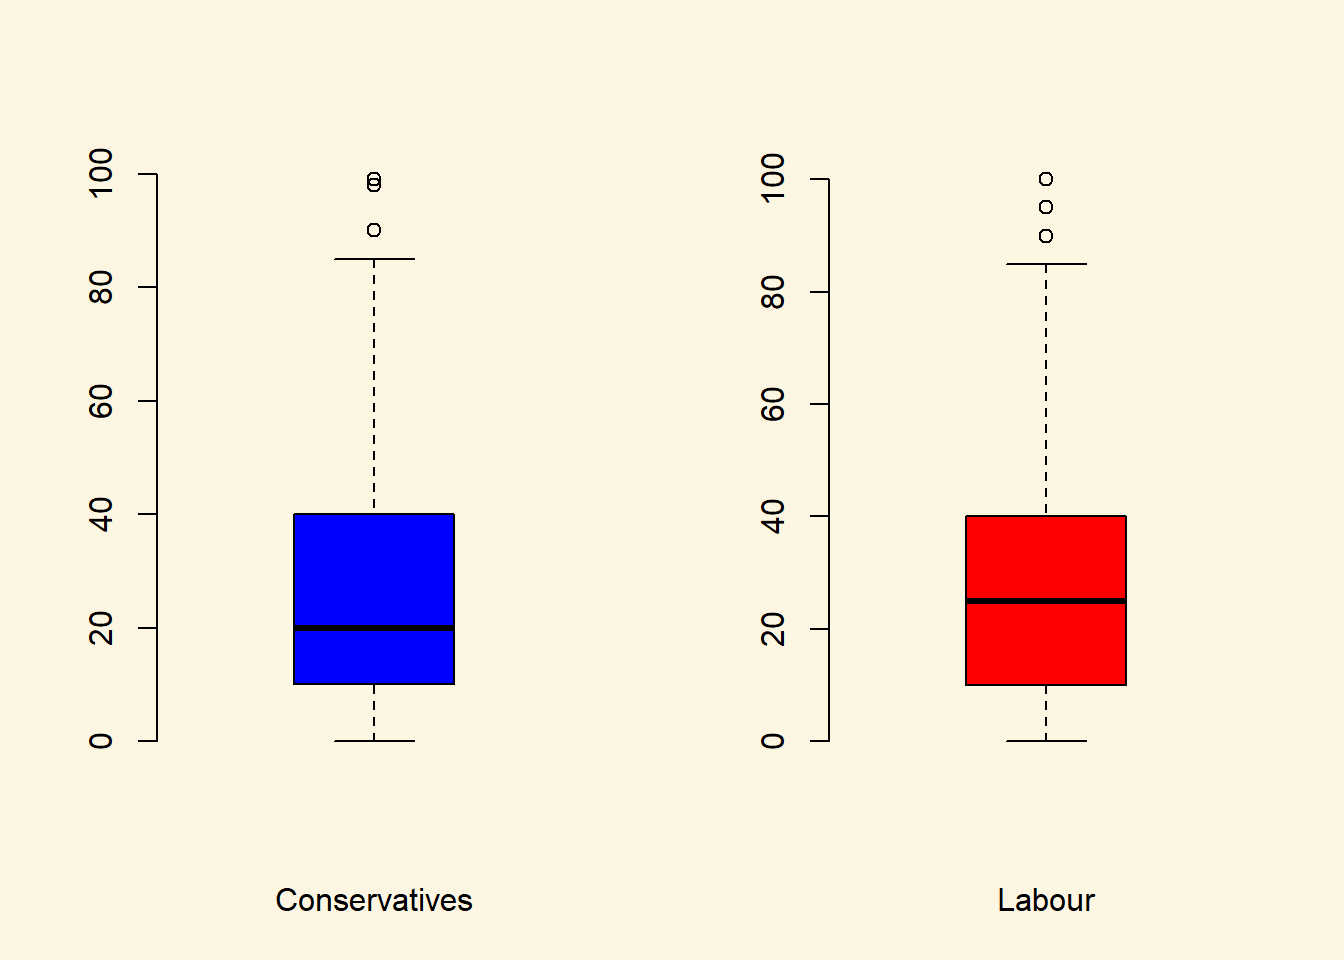
\includegraphics{stats101_files/figure-latex/unnamed-chunk-93-1.pdf}

We can see by looking at the regression line that it matches the coefficients we estimated above. For example, when \texttt{PctNotHSGrad} is equal to zero (i.e.~where the line intersects the Y-axis), the predicted value for \texttt{PctUnemployed} seems to be above 0 but below 10. This is good, as the \emph{intercept} coefficient we estimated in the regression was 7.8952023.

Similarly, the coefficient for the variable \texttt{PctNotHSGrad} was estimated to be 0.7423853, which implies that a one point increase in the percentage of citizens with no high-school education is associated with about 0.7423853 of a point increase in the percentage of citizens who are unemployed. The line in the plot seems to reflect this: it is upward sloping, so that higher levels of the no high-school variable are associated with higher levels of unemployment, but the relationship is not quite 1-to-1. That is, for each additional percentage point of citzens without high school education, the percentage of citizens who are unemployed increases by a little less than one point.

\hypertarget{multivariate-linear-regression}{%
\subsubsection{Multivariate linear regression}\label{multivariate-linear-regression}}

We might be interested in other variables that could explain the outcome. For instance, unemployment may be explained whether an community has a high urban population. For example, a more urban population may have better access to jobs.

Again we need to change the scale of a variable of interest - urban populationx, so that it is more interpretable.

\begin{Shaded}
\begin{Highlighting}[]
\NormalTok{communities}\OperatorTok{$}\NormalTok{PctUrban <-}\StringTok{ }\NormalTok{communities}\OperatorTok{$}\NormalTok{population }\OperatorTok{*}\DecValTok{100}
\end{Highlighting}
\end{Shaded}

Now lets add this to the model.

\begin{Shaded}
\begin{Highlighting}[]
\NormalTok{model2 <-}\StringTok{ }\KeywordTok{lm}\NormalTok{(PctUnemployed }\OperatorTok{~}\StringTok{ }\NormalTok{PctNotHSGrad }\OperatorTok{+}\StringTok{ }\NormalTok{PctUrban, }\DataTypeTok{data =}\NormalTok{ communities)}
\KeywordTok{summary}\NormalTok{(model2)}
\end{Highlighting}
\end{Shaded}

\begin{verbatim}

Call:
lm(formula = PctUnemployed ~ PctNotHSGrad + PctUrban, data = communities)

Residuals:
    Min      1Q  Median      3Q     Max 
-41.203  -8.372  -1.274   7.399  57.474 

Coefficients:
             Estimate Std. Error t value Pr(>|t|)    
(Intercept)   7.17377    0.64909  11.052  < 2e-16 ***
PctNotHSGrad  0.73651    0.01480  49.748  < 2e-16 ***
PctUrban      0.16436    0.02362   6.957 4.69e-12 ***
---
Signif. codes:  0 '***' 0.001 '**' 0.01 '*' 0.05 '.' 0.1 ' ' 1

Residual standard error: 13.36 on 1991 degrees of freedom
Multiple R-squared:  0.5636,    Adjusted R-squared:  0.5631 
F-statistic:  1286 on 2 and 1991 DF,  p-value: < 2.2e-16
\end{verbatim}

The coefficient for urban population is positive, which suggests a higher urban population increases unemployment. A one unit change in population increases unemployment by 1.64\%. Because this variable is at the same scale, we can compare this with the coefficient concerning the percentage of people without high school education. The p-value for this coefficient is also extremely low, meaning the estimate is statistically significant. Finally, we can see that the adjusted R-square has moved from 0.5527 to 0.5631 after adding the additional variable. This suggests the model is able to explain a bit more variation and has slightly more predictive power than the bivariate regression.

Let's plot the regression line:

\begin{Shaded}
\begin{Highlighting}[]
\KeywordTok{plot}\NormalTok{(}
  \DataTypeTok{x =}\NormalTok{ communities}\OperatorTok{$}\NormalTok{PctNotHSGrad,}
  \DataTypeTok{y =}\NormalTok{ communities}\OperatorTok{$}\NormalTok{PctUnemployed,}
  \DataTypeTok{xlab =} \StringTok{"Adults without high school education (%)"}\NormalTok{,}
  \DataTypeTok{ylab =} \StringTok{"Unemployment (%)"}\NormalTok{,}
  \DataTypeTok{frame.plot =} \OtherTok{FALSE}\NormalTok{,}
  \DataTypeTok{pch =} \DecValTok{20}\NormalTok{,}
  \DataTypeTok{col =} \StringTok{"LightSkyBlue"}
\NormalTok{)}
\KeywordTok{abline}\NormalTok{(model1, }\DataTypeTok{lwd =} \DecValTok{3}\NormalTok{, }\DataTypeTok{col =} \StringTok{"red"}\NormalTok{)}
\end{Highlighting}
\end{Shaded}

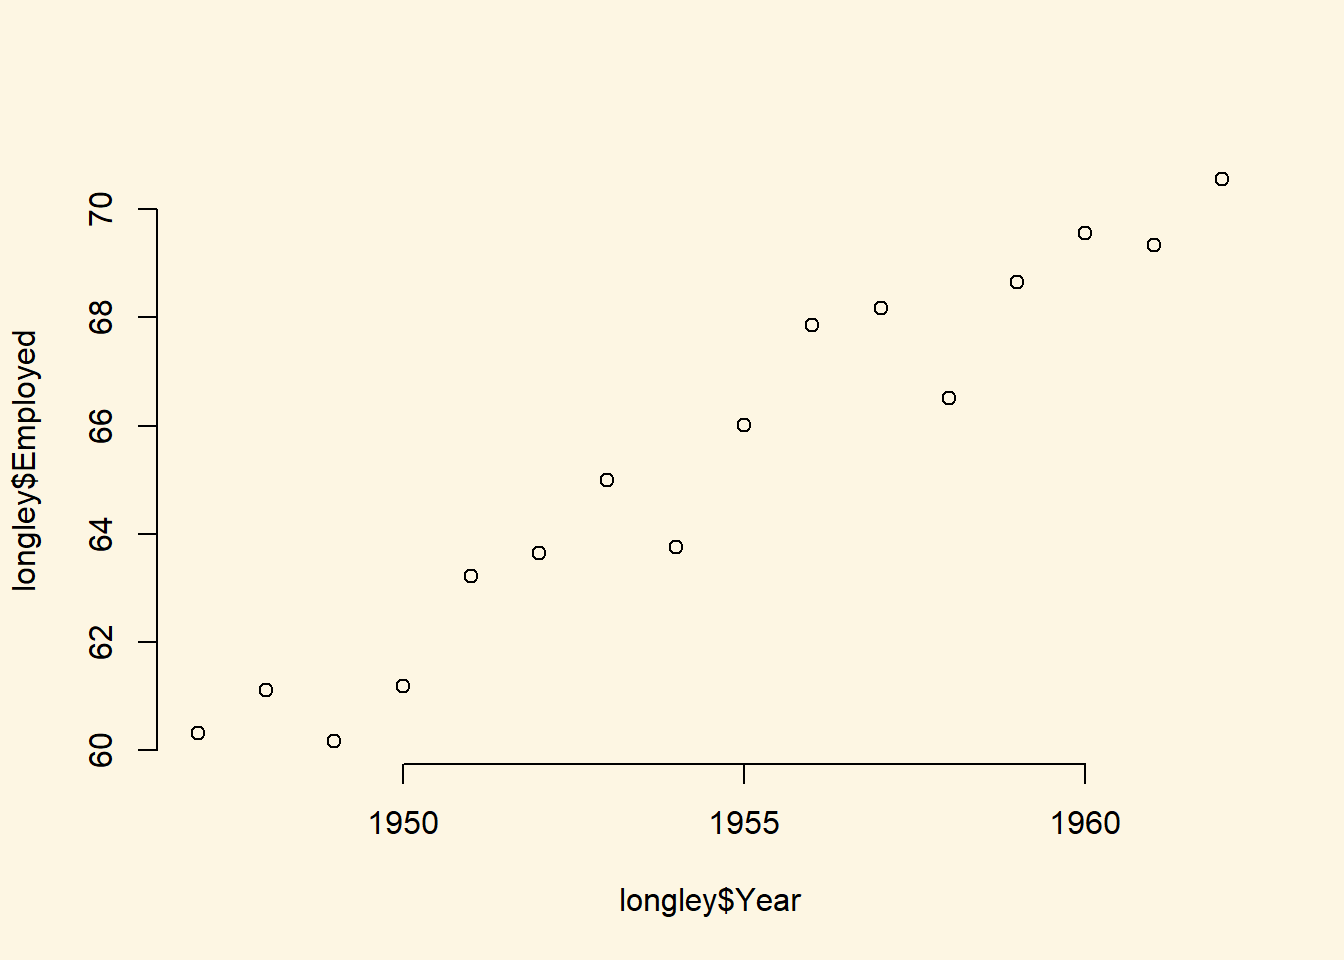
\includegraphics{stats101_files/figure-latex/unnamed-chunk-96-1.pdf}

As you can see from the plot, there are strange observations at the top of the y-axis and x-axis. This is strange as no observations with no education are likely to have 100\% employment. These outliers or incorrect values will bias the results, so lets run another model without these high values using subsetting:

\begin{Shaded}
\begin{Highlighting}[]
\NormalTok{model3 <-}\StringTok{ }\KeywordTok{lm}\NormalTok{(PctUnemployed }\OperatorTok{~}\StringTok{ }\NormalTok{PctNotHSGrad }\OperatorTok{+}\StringTok{ }\NormalTok{PctUrban, }
             \DataTypeTok{data =}\NormalTok{ communities [communities}\OperatorTok{$}\NormalTok{PctUnemployed }\OperatorTok{<}\StringTok{ }\DecValTok{100} 
                          \OperatorTok{&}\StringTok{ }\NormalTok{communities}\OperatorTok{$}\NormalTok{PctNotHSGrad }\OperatorTok{<}\DecValTok{100}\NormalTok{ , ])}
\KeywordTok{summary}\NormalTok{(model3)}
\end{Highlighting}
\end{Shaded}

\begin{verbatim}

Call:
lm(formula = PctUnemployed ~ PctNotHSGrad + PctUrban, data = communities[communities$PctUnemployed < 
    100 & communities$PctNotHSGrad < 100, ])

Residuals:
    Min      1Q  Median      3Q     Max 
-38.832  -8.043  -1.301   7.264  55.962 

Coefficients:
             Estimate Std. Error t value Pr(>|t|)    
(Intercept)   8.61368    0.64421  13.371  < 2e-16 ***
PctNotHSGrad  0.68359    0.01528  44.745  < 2e-16 ***
PctUrban      0.17304    0.02269   7.626 3.77e-14 ***
---
Signif. codes:  0 '***' 0.001 '**' 0.01 '*' 0.05 '.' 0.1 ' ' 1

Residual standard error: 12.78 on 1948 degrees of freedom
Multiple R-squared:  0.5204,    Adjusted R-squared:   0.52 
F-statistic:  1057 on 2 and 1948 DF,  p-value: < 2.2e-16
\end{verbatim}

This drops the coefficient slightly for the level of education attainment. What this means is the effect (or the slope of the regression line) on unemployment is reduced. However, the result is still statistically significant as the p-value is less than 0.05.

\hypertarget{additional-resources}{%
\subsubsection{Additional Resources}\label{additional-resources}}

\begin{itemize}
\tightlist
\item
  \href{http://altaf.shinyapps.io/linear-regression}{Linear Regression - Interactive App}
\end{itemize}


\end{document}
